\documentclass[openany]{book}

\usepackage{graphicx,epsfig}
\usepackage{hyperref}
\usepackage{amsmath,amssymb}
\usepackage[toc,page]{appendix}
\usepackage{longtable}
\usepackage{array}
\usepackage{float}
\usepackage{parskip}


\renewcommand{\baselinestretch}{1}

\setlength{\textheight}{9in}
\setlength{\textwidth}{6.5in}
\setlength{\headheight}{0in}
\setlength{\headsep}{0in}
\setlength{\topmargin}{0in}
\setlength{\oddsidemargin}{0in}
\setlength{\evensidemargin}{0in}
\setlength{\parindent}{.3in}
\pagestyle{plain}

\raggedbottom

\begin{document}
\bibliographystyle{plain}

\large

\thispagestyle{empty}
\centerline{\bf A REPORT}
\vspace*{0.3cm}
\centerline{\bf ON}
\vspace*{0.3cm}
\centerline{\bf EMPIRICAL ANALYSIS OF INVESTOR PROTECTION AND ASSET RECLAMATION:} % enter here
\centerline{\bf EVALUATING THE IEPFA FRAMEWORK (2016--2026)}
\vspace*{2cm}

\centerline{BY}
\vspace*{1cm}

\begin{center}
	\begin{tabular}{lll} % enter here
		Name(s) of the students & \hspace*{2cm} ID No(s). & \hspace*{2cm} Discipline(s) \\ 
		Soumya Banthia &\hspace*{2cm} 2024B3A71049G &\hspace*{2cm} M. Sc. in Economics \\

	\end{tabular}
\end{center}

\vspace*{2cm}
\begin{center}
	{\bf Prepared in partial fulfillment of the \\
	Practice School - I} \\ % enter here
\end{center}

\vspace*{0.5cm}

\centerline{AT}

\vspace*{1cm}
        \centerline{\bf National Council of Applied Economic Research, Delhi} % enter here
	\vspace{0.2cm}
	\centerline{\bf A Practice School - I}
	\vspace{0.2cm}
	\centerline{\bf Station of}
	\vspace{0.5cm}
\begin{figure}[ht]
\epsfxsize=1.0in
\centerline{\epsffile{logo.eps}}
\end{figure}

	\centerline{\bf BIRLA INSTITUTE OF TECHNOLOGY \& SCIENCE, PILANI}
	\vspace*{0.5cm}
	\centerline{\bf June, 2026} % enter here
	\newpage

\thispagestyle{empty}

	\centerline{\bf BIRLA INSTITUTE OF TECHNOLOGY \& SCIENCE, PILANI}
	\vspace*{0.2cm}
	\centerline{\bf Practice School Division}
	\vspace*{0.3cm}
	{\bf 
	%\begin{center}
		\begin{tabular}{p{6cm}l}
			& \\
			& \\
			& \\
			Station & \hspace*{3cm} Centre \\  NCAER & \hspace*{3cm} Delhi
			& \\
			Duration &\hspace*{3cm} Date of start \\ 8 Weeks & \hspace*{3cm} 25-06-2026
			& \\
			Date of submission & {} \\  20-06-2026 \\
			& \\
			Title of the project: & \\ \parbox[t]{15 cm} {Empirical Analysis of Investor Protection and Asset Reclamation: Evaluating the IEPFA Framework (2016--2026)} \\
			& \\
			ID No.(s), Name(s) and Disciplines of the student(s): & \\ \parbox[t]{15 cm} {2024B3A71049G, Soumya Banthia, M. Sc. in Economics} \\
            & \\
			Name(s) and Designation(s) of the expert(s): & \\ \parbox[t]{15 cm} {C S Mohapatra, IEPF Chair Professor} \\
			& \\ 
			Name(s) of the PS faculty member(s): & \\ Mohit Kumar \\
            & \\ 
			Key words: & \\ \parbox[t]{15 cm} {Investor Protection, Unclaimed Financial Assets, Household Finance, Financial Regulation, Regulatory Digitization, Empirical Econometrics} \\
			& \\
			Project area(s):  & \\ \parbox[t]{15 cm} {Empirical Finance, Financial Regulation, Household Economics, and Law \& Economics}\\
			& \\
			Abstract: & \\ \parbox[t]{16 cm} {This study provides an empirical and institutional evaluation of the Investor Education and Protection Fund Authority (IEPFA) over the period 2016--2026. Utilizing a 10-year longitudinal panel of statutory corporate compliance filings (Forms IEPF-1 through IEPF-7), fund accumulation metrics, and nationwide Investor Awareness Program (IAP) interventions, we investigate frictional costs in asset reclamation and the impact of regulatory digitization. Applying a Difference-in-Differences (DiD) and fixed-effects framework around the 2019 Process Re-engineering reforms, we document that the transition to PAN-verified digital claim processing substantially increased claim resolution efficiency and filing volumes. Furthermore, physical grassroots literacy campaigns exhibit positive elasticities with respect to retail investor participation. Finally, we benchmark India's unclaimed property architecture against international regimes (US NAUPA, UK Dormant Assets Scheme, and German BGB/BaFin) and propose targeted regulatory enhancements for capital market integrity.}\\
			& \\
            Soumya Banthia\\
			Signature of the student(s) & \hspace*{1cm}Signature of the PS faculty member(s) \\
			& \\
			Date & \hspace*{1cm}Date \\ 20-06-2026
		\end{tabular}}

	\newpage
	\centerline{\bf \Large Acknowledgements}
	\vspace*{0.5cm}
		\par\noindent 

I would like to express my sincere gratitude to Dr. C. S. Mohapatra, IEPF Chair Professor at the National Council of Applied Economic Research (NCAER), for providing me with the opportunity to work on this project and for his valuable guidance, encouragement, and continuous support throughout my Practice School programme. \\
        
I am also thankful to Mr. Mohit Kumar, my Practice School faculty member from BITS Pilani, for his guidance and constructive suggestions during the course of the project.\\
        
I would like to acknowledge the support of the researchers and staff at NCAER for providing the necessary resources and a conducive learning environment. Their insights and assistance have been invaluable in understanding the concepts of Investor Protection and Financial Regulation.\\
        
Finally, I express my heartfelt gratitude to my family and friends for their constant encouragement and support throughout this journey.
		
		\vfill

        Soumya Banthia \\ 
		\par\noindent {\bf Signature of the student(s)}

\tableofcontents
\listoffigures
\listoftables

\chapter{Introduction}

\section{Economic Motivation and Background}
In modern market economies, capital markets rely on transparent governance, investor trust, and efficient clearing and custody mechanisms \cite{guiso2008trusting, zingales2009future}. However, a pervasive yet understudied friction in retail equity and bond markets is the phenomenon of \textit{dormant and unclaimed financial assets}. When dividends, matured debentures, share certificates, or redemption proceeds remain unclaimed over prolonged horizons, they generate substantial deadweight losses. For households, dormant assets represent lost wealth and suboptimal consumption smoothing \cite{campbell2006household}. For issuing corporations, holding unclaimed balances indefinitely on balance sheets introduces custodial agency problems, compliance burdens, and accounting opacity.

To address these inefficiencies, institutional mechanisms are required to disintermediate dormant capital, protect property rights, and channel accumulated funds into public goods such as investor awareness and systemic financial literacy. In India, this institutional function is governed by the Investor Education and Protection Fund Authority (IEPFA), a statutory body established by the Government of India on 7th September 2016 under Section 125 of the Companies Act, 2013, under the administrative purview of the Ministry of Corporate Affairs (MCA).

The origin of the fund traces back to Section 205C of the Companies Act, 1956, introduced via the Companies (Amendment) Act, 1999. While the 1956 framework established the basic principle that unclaimed company dividends should transfer to a public fund after seven consecutive years, it lacked an autonomous administrative apparatus and sophisticated technological verification architecture. Consequently, billions of rupees in unclaimed corporate dividends remained fragmented across thousands of individual corporate accounts. The enactment of Section 125 of the Companies Act, 2013, and the subsequent operationalisation of the IEPFA in 2016 marked a structural shift toward centralised custody, rigorous digital verification, and targeted investor restitution.

\section{Statutory and Legal Mandates (Section 125, Companies Act 2013)}
Section 125 of the Companies Act, 2013 establishes both the Fund and the Authority with a dual statutory mandate:
\begin{enumerate}
    \item \textbf{Fiduciary Custody and Asset Restitution:} Under Section 124(5) and Section 125(2), any dividend unpaid or unclaimed for seven consecutive years, along with the underlying shares (Section 124(6)), must be transferred by corporate entities to the Fund. The Authority acts as a sovereign trustee, verifying legitimate investor claims via Form IEPF-5 and releasing disgorged amounts and underlying equity back to rightful claimants or their legal heirs.
    \item \textbf{Financial Literacy and Investor Advocacy:} Under Section 125(3)(b), the Fund is explicitly deployed to promote investor education and protection. The income accrued on fund investments is utilized to conduct nationwide Investor Awareness Programs (IAPs), publish empirical research, finance Chair Professorships at premier think tanks (such as NCAER and IICA), and run multilingual multimedia advocacy campaigns.
\end{enumerate}

\section{Research Objectives and Empirical Hypotheses}
This report provides a data-driven evaluation of IEPFA's institutional evolution and operational performance across its first full decade of existence (2016--2026). Specifically, this study investigates three central research questions:
\begin{itemize}
    \item \textbf{Research Question 1 (Regulatory Digitization and Disposal Efficiency):} Did the 2019 Process Re-engineering reforms (introduction of web-based Form IEPF-5, PAN-linked e-verification, and elimination of physical share certificate collection) causally reduce bureaucratic friction and increase claim disposal velocity?
    \item \textbf{Research Question 2 (Grassroots Outreach Elasticity):} How effective are targeted, physical investor awareness campaigns (such as \textit{Niveshak Didi} postal initiatives and \textit{Niveshak Sarathi} mobile vans) relative to broad digital and broadcast campaigns in generating retail investor engagement and asset reclamation?
    \item \textbf{Research Question 3 (Institutional Transparency):} How has the statutory grievance and information dissemination mechanism evolved, as measured by Right to Information (RTI) disposal rates and first-appeal ratios?
\end{itemize}

\section{Structure of the Report}
The remainder of this report is organized as follows: Chapter 2 reviews the academic literature on household finance, behavioral frictions, and international comparative frameworks, alongside the regulatory notifications governing the IEPFA. Chapter 3 outlines the empirical methodology, econometrics specification (Difference-in-Differences and Panel Fixed Effects), and dataset construction. Chapter 4 presents comprehensive empirical findings across e-form filing volumes, accumulation dynamics, share restitution, and RTI transparency. Chapter 5 concludes with systemic insights, and Chapter 6 articulates actionable policy and technological recommendations for future capital market governance.

\chapter{Literature review}

\section{Theoretical Foundations: Household Finance and Asset Dormancy}
The study of unclaimed financial assets lies at the intersection of household portfolio choice, behavioral economics, and regulatory architecture. In classical financial economics, households optimize intertemporal consumption and investment portfolios under the life-cycle hypothesis \cite{campbell2006household}. However, empirical household finance documents pervasive non-standard behaviors: inertia, under-diversification, and extreme dormancy in financial claims \cite{beshears2018behavioral}.

Asset dormancy emerges primarily from three core frictions:
\begin{enumerate}
    \item \textbf{Informational Asymmetry and Rational Inattention:} Investors face search and tracking costs across multiple equity registries, corporate registrars and transfer agents (RTAs), and depository participants. When dividends are small relative to transaction and bureaucratic search costs, rational inattention leads households to abandon tracking fractional disbursements.
    \item \textbf{Cognitive Friction and Financial Literacy Gaps:} As demonstrated by \cite{lusardi2014financial}, low financial literacy severely hinders households' ability to navigate complex probate, transmission, and succession procedures when original shareowners pass away intestate.
    \item \textbf{Institutional and Search Frictions:} Physical share certificates and outdated corporate address registries create friction in asset transfer, allowing corporate dividends to accumulate unclaimed for years.
\end{enumerate}

From a Law and Finance perspective, legal origins and statutory enforcement mechanisms strongly dictate the degree of investor protection and market depth \cite{la1998law}. Regulatory regimes that establish credible custodial funds reduce the expropriation risk of minority retail shareholders by corporate managers \cite{zingales2009future, guiso2008trusting}.

\section{International Comparative Frameworks for Unclaimed Property}
Regulatory mechanisms for managing unclaimed capital market balances vary across advanced and emerging economies. Table \ref{tab:international_comparison} provides a comparative synthesis of statutory regimes across the United States, the United Kingdom, Germany, and India.

\begin{table}[H]
\centering
\small
\begin{tabular}{|p{3cm}|p{3.5cm}|p{3.5cm}|p{3.8cm}|}
\hline
\textbf{Jurisdiction} & \textbf{Statutory Authority / Legal Basis} & \textbf{Dormancy Horizon \& Custody Regime} & \textbf{Utilization of Accumulated Funds / Restitution Rights} \\ \hline
\textbf{United States} & State Treasuries / NAUPA (Uniform Unclaimed Property Act) & Typically 3--5 years; Escheatment to state general treasury in perpetuity. & Held in custodial trust; funds can be borrowed by state for public infrastructure; claims never expire. \\ \hline
\textbf{United Kingdom} & Dormant Assets Scheme / Reclaim Fund Ltd (RFL) & 15 years for bank accounts; expanded to investment assets and pensions. & Allocated to social and environmental causes via National Lottery Community Fund; full right of reclaim preserved. \\ \hline
\textbf{Germany / EU} & German Civil Code (\S 195, \S 199 BGB) / BaFin & 3-year standard statute of limitations; no centralised custodial state fund for equity. & Reverts to holding financial institutions/issuers after prescription period unless fraud is proven; decentralized restitution. \\ \hline
\textbf{India} & IEPFA (Section 125, Companies Act, 2013) & 7 consecutive years; centralized transfer of unpaid dividends and underlying equity. & Sovereign custodial fund; returns accrued on investments fund mandatory financial education programs; perpetual restitution rights. \\ \hline
\end{tabular}
\caption{International Comparative Matrix of Unclaimed Asset Governance}
\label{tab:international_comparison}
\end{table}

\section{Organisational Structure} \cite{iepfa_annual_reports}
\begin{figure}[h]
    \centering
    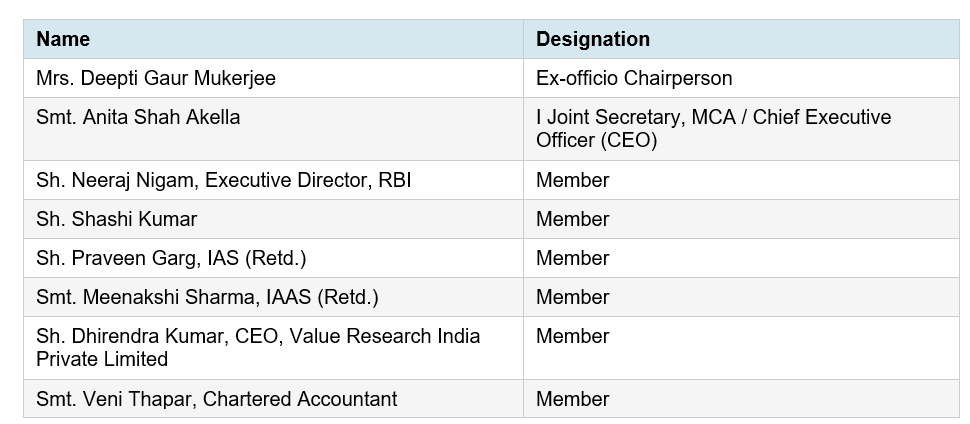
\includegraphics[width=0.8\textwidth]{image1.png}
    \caption{Present members and Chairperson of IEPFA}
    \label{fig:iepfa_members}
\end{figure}
\begin{figure}[h]
    \centering
    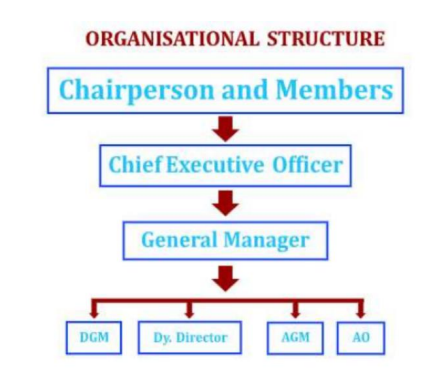
\includegraphics[width=0.4\textwidth]{image2.png}
    \caption{Organisational Hierarchy of IEPFA}
    \label{fig:iepfa_hierarchy}
\end{figure}

\section{Legal and Regulatory Framework} \cite{iepfa_annual_reports}
\subsection{List of rules (GSR Notifications from 2016 to 2021)}
\begin{table}[H]
\centering
\begin{tabular}{|p{3cm}|p{2.5cm}|p{10cm}|}
\hline
\textbf{GSR No.} & \textbf{Date} & \textbf{Rules} \\ \hline
G.S.R. 26(E) & 13.01.2016 & Investor Education and Protection Fund Authority (Appointment of Chairperson and Members, holding of meetings and provision for offices and officers) Rules, 2016. \\ \hline
G.S.R. 854(E) & 05.09.2016 & Investor Education and Protection Fund Authority (Accounting, Audit, Transfer and Refund) Rules, 2016. \\ \hline
G.S.R. 46(E) & 18.01.2017 & Investor Education and Protection Fund Authority (Recruitment, Salary and other Terms and Conditions of Service of General Manager and Assistant General Manager) Rules, 2017. \\ \hline
G.S.R. 178(E) & 28.02.2017 & Investor Education and Protection Fund Authority (Accounting, Audit, Transfer and Refund) Amendment Rules, 2017. \\ \hline
G.S.R. 1267(E) & 13.10.2017 & Investor Education and Protection Fund Authority (Accounting, Audit, Transfer and Refund) Second Amendment Rules, 2017. \\ \hline
G.S.R. 472(E) & 22.05.2018 & Investor Education and Protection Fund Authority (Accounting, Audit, Transfer and Refund) Third Amendment Rules, 2017 \\ \hline
G.S.R. 793(E) & 21.08.2018 & Investor Education and Production fund Authority (Recruitment, Salary and other Terms and Conditions Of services of Deputy General Manager, Private Secretary, Personal Assistant, Stenographer, Senior Secretariat Assistant and Junior Secretariat Assistant Recruitment) Rules, 2018. \\ \hline
G.S.R. 1023(E) & 11.10.2018 & Investor Education and Protection Fund Authority (Form of Annual Statement of Accounts) And (Form and Time of Preparation of Annual Report) Rules, 2018. \\ \hline
G.S.R.343(E) & 01.05.2019 & Investor Education and Protection Fund Authority (Accounting, Audit, Transfer and Refund) Amendment Rules, 2019 \\ \hline
G.S.R.571(E) & 14.08.2019 & Investor Education and Protection Fund Authority (Accounting, Audit, Transfer and Refund) Second Amendment Rules, 2019 \\ \hline
G.S.R.702(E) & 30.09.2019 & Investor Education and Protection Fund Authority (Recruitment, Salary and other Terms and Conditions of Service of General Manager and Assistant General Manager) Amendment Rules, 2019 \\ \hline
G.S.R.703(E) & 30.09.2019 & Investor Education and Protection Fund Authority (Recruitment, Salary and other Terms and Conditions of Service of Deputy General Manager, Private Secretary, Personal Assistant, Stenographer, Senior Secretariat Assistant (SSA) and Junior Secretariat Assistant (JSA)) Amendment Rules, 2019 \\ \hline
General Circular No.35/2020 & 29.09.2020 & Fillings under section 124 and section 125 of the Companies Act 2013 r/w IEPFA (Accounting, Audit, Transfer and Refund) Rules 2016 in view of extension of CFSS, 2020 \\ \hline
G.S.R. 396 (E) & 09.06.2021 & Investor Education and Protection Fund Authority (Accounting. Audit, Transfer and Refund) Amendment Rules, 2021 \\ \hline
G.S.R. 785 (E) & 09.11.2021 & Investor Education and Protection Fund Authority (Accounting, Audit. Transfer and Refund) Second Amendment Rules, 2021 \\ \hline
G.S.R. 888(E) & 28.12.2021 & Investor Education and Protection Fund Authority (Accounting, Audit, Transfer and Refund), Third Amendment, Rules, 2021 \\ \hline
\end{tabular}
\caption{List of GSR Notifications and Rules}
\label{tab:gsr_rules}
\end{table}

\subsection{List of e-Forms }
\begin{table}[H]
\centering
\begin{tabular}{|p{3.5cm}|p{11.5cm}|}
\hline
\textbf{Form} & \textbf{Description} \\ \hline
IEPF Form- 1 & Statement of amounts credited to Investor Education and Protection Fund \\ \hline
IEPF Form-2 & Statement of unclaimed and unpaid amounts \\ \hline
IEPF Form-1A & Statement of Amounts credited to Investor Education and Protection Fund Pursuant to Rule 5 (4A)-Introduced vide Notification GSR 571(E) dated 14th August 2019 \\ \hline
IEPF Form-3 & Statement of shares and unclaimed or unpaid dividend not transferred to the Investor Education and Protection Fund \\ \hline
IEPF Form-4 & Statement of shares transferred to the Investor Education and Protection Fund \\ \hline
IEPF Form-5 & Application to the authority for claiming unpaid amounts and shares out of the Investor Education and Protection Fund \\ \hline
IEPF Form-6 & Statement of unclaimed or unpaid amounts to be transferred to the Investor Education and Protection Fund-Deprecated vide Notification GSR571(E) dated 14th August 2019 \\ \hline
IEPF Form-7 & Statement of amounts credited to IEPF on account of shares transferred to the fund \\ \hline
\end{tabular}
\caption{List of e-Forms}
\label{tab:e_forms}
\end{table}

\section{Process re-engineering reforms (2019 amendments)} \cite{iepfa_annual_reports}
Based on the recommendations of a committee member, amendments in IEPF Rules, 2016 came into effect vide notification of Investor Education and Protection Fund
Authority (Accounting, Audit, Transfer and Refund) Second Amendment Rules, 2019, dated August 14, 2019. The major recommendations that were implemented are as
follows:
\begin{itemize}
    \item Claim settlement process -
    \begin{itemize}
        \item A new simplified web-based e-form IEPF-5, having features of PAN-based verification, was implemented. 
        \item The processing of e-form IEPF 5 by the companies and submission of verification reports to the Authority was made online. 
        \item The practice of collecting physical share certificates from the claimants was discontinued, and only a scanned copy of cancelled certificates is obtained from the companies along with the online verification report. 
    \end{itemize}  
    \item Collection of investor-wise data for the period before the constitution of the Authority - For the period before 2006, the information about shareholders/investors whose amounts have been transferred was not available in The MCA 21 system, a new form IEPF -1A was made available. \\
    \item Online appointment and updating of Nodal/Deputy Nodal Officer data - Companies were enabled to appoint Nodal/Deputy Nodal Officers for processing of IEPF-related claims through form IEPF-2. The details of the nodal officer of the Company are displayed on the website of the Companies & Authority. Further, the year-wise details of funds that were to be transferred to IEPF were collected through the form. \\
    \item  Standard documents list and Standard Operating Procedure - Standard document list and Standard Operating Procedure for processing of claims including those involving transmission and loss of share certificates, were prescribed through Schedules. 
    
\end{itemize}

\section{Sources of credits to IEPF}
As per section 125(2) of the Companies Act 2013, there shall be credited to the Fund: 
\begin{itemize}
    \item (a) the amount given by the Central Government by way of grants after due appropriation made by Parliament by law in this behalf for being utilized for the purposes of the Fund;  
    \item (b) donations given to the Fund by the Central Government, State Governments, companies or any other institution for the purposes of the Fund;  
    \item (c) the amount in the Unpaid Dividend Account of companies transferred to the Fund under sub-section (5) of section 124;  
    \item (d) the amount in the general revenue account of the Central Government which had been transferred to that account under sub-section (5) of section 205A of the Companies Act, 1956, as it stood immediately before the commencement of the Companies (Amendment) Act, 1999, and remaining unpaid or unclaimed on the commencement of this Act;  
    \item (e) the amount lying in the Investor Education and Protection Fund under section 205C of the Companies Act, 1956;  
    \item (f) the interest or other income received out of investments made from the Fund;  
    \item (g) the amount received under sub-section (4) of section 38; 
    \item (h) The application money received by companies for allotment of any securities and due for refund.  
    \item (i) matured deposits with companies other than banking companies; 
    \item (j) matured debentures with companies.  
    \item (k) interest accrued on the amounts referred to in clauses (h) to (j);  
    \item (l) sale proceeds of fractional shares arising out of the issuance of bonus shares, merger and amalgamation for seven or more years;  
    \item (m) redemption amount of preference shares remaining unpaid or unclaimed for seven or more years; and  
    \item (n) such other amount as may be prescribed: Provided that no such amount referred to in clauses (h) to (j) shall form part of the Fund unless such amount has remained unclaimed and unpaid for a period of seven years from the date it became due for payment.  
 
\end{itemize}

\section{Permitted Utilization of the Fund} \cite{iepfa_annual_reports}
According to Section 125(3) of the Companies Act, 2013, IEPF shall be utilised for the following: 
 
\begin{itemize}
    \item  Refund of unclaimed dividends, deposits, debentures and application money due for refund and the interest thereon. 
    \item  Promotion of investor education through awareness and financial literacy programmes and activities aimed at protecting investor interests. 
    \item Distribution of disgorged amounts among eligible and identifiable investors who have suffered losses due to wrongful action of any person, in accordance with court orders. 
    \item Reimbursement of legal expenses incurred in pursuing class action suits under section 37 and 245 of the Companies Act, 2013, as sanctioned by the tribunal. 
    \item Any other purpose incidental to the objectives of the fund, as may be prescribed under the relevant rules.  
    
\end{itemize}


\section{Claim Settlement} \cite{iepfa_annual_reports}

\subsection{Legal provisions}
Section 125 (4) of ``The Companies Act, 2013'' provides that any person claiming to be entitled to the amount referred in sub-section (2) of section 125 may apply to the Authority for the payment of amount claimed. Further, Section 124 (6) of the Companies Act, 2013 provides that any claimant of shares transferred to the fund shall be entitled to claim the transfer of shares from IEPF.

\subsection{Step-by-step claim process}
\begin{itemize}
    \item File an online application in Form IEPF-5 seeking a refund from the authority.
    \item Send the form along with the requisite documents as enumerated in Form IEPF-5 to the concerned company at its registered office for verification of the claim.
    \item The Company is required to send an online verification report to the authority within thirty days, along with a scanned copy of the documents submitted by the claimant through the MCA 21 IT system.
    \item An application complete in all respects is required to be disposed of by the authority within sixty days from the date of receipt of the verification report and other relevant documents from the company.
    \item The Authority processes those claims where the IEPF-5 form is filed, along with complete and correct documentation, and an approved e-verification report from the Nodal officer is received. In some cases, the Company Nodal Officer sends a rejected e-verification report, in which case the claim is rejected by the Authority. Incomplete or defective claims/documents are returned to the Company to correct the discrepancies. (Every Company has their own process to verify the documents.)
    \item Notices are issued to Companies in cases where e-verification reports for a claim have not been received.
    \item After expiry of the notice period, in case of no response, the claims are rejected.
\end{itemize}

\subsection{Process re-engineering highlights (2019)}
\begin{itemize}
    \item A new simplified web-based e-form IEPF-5 having features of PAN-based verification was implemented.
    \item The processing of e-form IEPF 5 by the companies and submission of verification reports to the Authority was made online.
    \item The practice of collection of physical share certificates from the claimants was discontinued, and only a scanned copy of cancelled certificates was obtained from the companies, along with the online verification report.
    \item A new form IEPF -1A was made available to collect information about shareholders/investors whose amounts have been transferred for the period before 2006.
    \item Companies were enabled to appoint Nodal/Deputy Nodal Officers for processing of IEPF-related claims through Form IEPF-2. The year-wise details of funds that are to be transferred to IEPF are collected through the form.
    \item Standard document list and Standard Operating Procedure for processing of claims, including those involving transmission and loss of share certificates, were prescribed through Schedules.
\end{itemize}

\subsection{Helpline Details}
The IEPFA Call Centre Help Line 14453 and office number 011-23441777 facilitates the investors. A Help Line (Call Centre) developed with the help of CSC e-Gov Services India is being used for addressing the queries of claimants. Citizens can also report suspicious claims on the Helpline and at the IEPF portal (\url{www.iepfportal.in}).



\section{Investor Awareness Programmes (IAPs)} \cite{iepfa_annual_reports} & \cite{iepfa_linkedin_posts} & \cite{iepfa_x_profile}

\subsection{FY 2019-20}
\begin{enumerate}
    \item \textbf{IAPs through Common Service Centers (CSC SPV):} Conducted to spread investor awareness in rural areas where professional institutes had limited reach. MoU was signed with CSC e-Governance Services India Ltd. (MeitY) to organize IAPs through CSC centers across rural India.
    \item \textbf{MoU with Nehru Yuva Kendra Sangathan (NYKS):} Signed on October 16, 2019, to leverage NYKS's youth network for last-mile investor awareness. A pilot project was proposed for 50 districts, 250 blocks, and 2,500 villages across 8 northern states, with Training of Trainers conducted for NYKS district coordinators.
    \item \textbf{Collaboration with India Post Payments Bank (IPPB):} To utilize IPPB's vast postal network for financial literacy camps. MoA signed for 4,404 Investor Awareness and Financial Literacy Camps across 23 postal circles and 650 branches covering all states from May to July 2020.
    \item \textbf{MoU with Bank of Baroda:} Signed on December 4, 2019, to co-brand IEPFA collaterals across the bank's marketing channels at no cost. Enabled placement of investor awareness posters in bank branches, digital banners in ATMs, and IEPFA messages on passbooks and welcome kits.
    \item \textbf{MoU with ICICI Bank:} Signed on March 18, 2020, to enhance dissemination of investor awareness information via digital collateral. Expanded IEPFA's digital outreach through the bank's digital platforms.
    \item \textbf{MoU with Kotak Mahindra Bank:} Signed on March 26, 2020, to co-brand investor awareness content in print and digital channels. Increased IEPFA's reach among the bank's customer base at no cost.
    \item \textbf{State-Level Conferences with Professional Institutes:} Organized to highlight investor education and self-employment opportunities in finance. Conferences held in Bhubaneswar (September 2019) and Dharamshala (December 2019), inaugurated by Union Minister Anurag Singh Thakur, engaging students, NYKS volunteers, and industry stakeholders.
    \item \textbf{IAPs through Professional Institutes (ICAI, ICSI, ICoAI):} To promote investor awareness in urban and semi-urban areas through trusted professional bodies. Programmes organized by local chapters and empaneled resource persons across cities, covering investment, savings, and market awareness.
    \item \textbf{Association with IICA as Knowledge Partner:} Engaged IICA to build a scalable, expert-led resource ecosystem for investor education. Over 300 resource persons were empanelled, Training of Trainers conducted, and new investor education modules developed for various stakeholder segments.
\end{enumerate}

\subsection{FY 2020-21}
\begin{enumerate}
    \item \textbf{IAPs through CSC SPV in 117 Aspirational Districts:} To reach rural citizens, especially women, farmers, and marginalized sections in aspirational districts, focusing on financial inclusion. 4,034 IAPs were conducted across 99 districts of 28 states, covering 1,83,150 rural citizens through mobilization via calls, WhatsApp, and door-to-door visits.
    \item \textbf{Investor Awareness by NYKS:} To sustain investor awareness momentum through youth volunteers despite COVID-19 restrictions. 16 webinars and digital IAPs were conducted until March 2021, engaging over 300 NYKS officials, national youth volunteers, and youth leaders.
    \item \textbf{Digital Literacy Camps by IPPB:} To continue investor education amid COVID-19 while observing social distancing norms. 108 physical/digital camps were organized by 23 circles; after pandemic relief, approximately 734 camps educated 55,000 citizens.
    \item \textbf{Collaboration with IndusInd Bank:} Extended bank co-branding partnerships to further widen IEPFA's outreach through IndusInd Bank's print and digital channels. MoU signed with IndusInd Bank in addition to existing collaborations with Bank of Baroda, Kotak Mahindra, and ICICI Bank.
    \item \textbf{Webinars by Professional Institutes (ICAI \& ICSI):} To maintain investor education continuity during lockdown using digital platforms. ICAI organized multiple webinars; ICSI held a national webinar on September 7, 2020, with senior MCA and IEPFA officials, drawing wide participation on a PAN India basis.
    \item \textbf{Scroll Messages on Doordarshan:} To leverage Doordarshan's mass reach for spreading investor awareness through passive exposure. Scroll messages were aired from September 2020, with an extension granted to Doordarshan (Prasar Bharti) from February 6, 2021.
    \item \textbf{Publicity Campaign on Lok Sabha TV:} To amplify IEPFA's message during the Parliament session for maximum policy-level visibility. Two video spots aired from September 17 to October 1, 2020, with additional AV spots during the budget session.
    \item \textbf{IEPFA Mobile App Launch:} To enhance citizen service delivery and grievance redressal through digital tools. The mobile app was launched by the Finance and Corporate Affairs Minister on March 25, 2021, alongside activation of IEPFA social media accounts and full adoption of e-office mode.
    \item \textbf{NCAER Workshops on Investor Education:} A five-part virtual workshop series to analyze investor education and protection strategies across financial sectors in India. Covered securities markets (December 28, 2020), insurance sector (January 20, 2021), national pension system (February 17, 2021), and AT1 bond disclosure impact (March 23, 2021), featuring RBI Governor and leading regulators.
\end{enumerate}

\subsection{FY 2021-22}
\begin{enumerate}
    \item \textbf{CSC SPV IAPs Across India:} To scale investor awareness to all rural areas beyond aspirational districts, covering the breadth of India. Completed the 15,000 IAP project in 117 aspirational districts, reaching 6,72,436 citizens; additionally, 10,966 ground IAPs were conducted, spreading financial literacy to 4,89,286 citizens despite COVID restrictions. IIT Delhi conducted an impact assessment.
    \item \textbf{NYKS Regional Orientation Programme, Chandigarh:} To train NYKS district officers to carry investor awareness to ground level post-pandemic. A two-day regional programme in December 2021 covered 17 districts with 20+ officers trained on savings, banking, government schemes, cybercrime awareness, and grievance redressal.
    \item \textbf{IPPB Financial Literacy Camps:} To continue camp-based financial literacy outreach after pandemic-era restrictions eased. Approximately 3,200 camps reached 1,21,545 citizens cumulatively; in this year alone, 2,212 IAPs were held, educating 59,224 citizens in vernacular languages.
    \item \textbf{MoU with ICAI:} Signed on December 13, 2021, to conduct IAPs for educated but financially unaware urban segments. ICAI conducted 66 IAPs in 3 months across cities including Ahmedabad, Ranchi, Meerut, and Cuttack, educating over 6,000 citizens on savings, banking, and investments.
    \item \textbf{IAPs with NCC Cadets:} To integrate investor awareness into youth development and early financial education. Interactive sessions were held at NCC Bhawan, Kirti Nagar and Rohini on November 26 and 29, 2021, covering topics such as savings, capital markets, and budgeting under Azadi ka Amrit Mahotsav.
    \item \textbf{IAPs at Gram Panchayats on Human Rights Day:} To align investor awareness with grassroots rights-based messaging and reach rural populations on a significant occasion. On December 10, 2021, 10 IAPs were held across Rajasthan Panchayats under Azadi Ka Amrit Mahotsav, educating 1,000+ locals on mutual funds, digital payments, and banking in local dialects.
    \item \textbf{ICSI National Webinar – IEPFA 5-Year Journey:} To celebrate and share IEPFA's achievements with a wide audience and chart future direction. Organized on September 7, 2021, with Union Minister of State for Corporate Affairs as Chief Guest; two technical sessions reviewed investor education milestones and roadmap to 2047.
    \item \textbf{MoU Renewal with ICICI Bank:} Signed on February 11, 2022, as an extension of the 2020 collaboration to deepen digital investor education. Covered training programmes, digital banking medium campaigns, and collaborative content, signed by GM IEPFA and ICICI Bank's Head of Strategic Relations.
    \item \textbf{IEPF Research Chairs at NCAER and IICA:} To institutionalize research on investor education and protection and build an evidence base for policy. Chairs established at both institutions to publish research, organize workshops, review national strategies, and improve the investor climate in India.
    \item \textbf{State-Level Conference at Guwahati, Assam:} To engage stakeholders across the Northeast in investor education and awareness. Held on March 29, 2022, with the Governor of Assam as Chief Guest; around 1,100 delegates including NCC cadets, students, ICSI and ICAI members, and government officials participated.
    \item \textbf{MoU with IGNOU for Gyan Darshan Tele-Lecture Series:} To use IGNOU's broadcast infrastructure to reach a wide youth audience through 75 educational episodes. Signed on January 12, 2022; a tele-lecture series on investor education was planned for airing on the 24x7 Gyan Darshan channel as part of Azadi Ka Amrit Mahotsav.
\end{enumerate}

\subsection{FY 2022-23}
\begin{enumerate}
    \item \textbf{Niveshak Didi (IPPB):} Launched to deliver financial literacy to rural women by trained female postmasters (Gramin Dak Sevaks), overcoming cultural and accessibility barriers. Under Phase I, 1,084 awareness programmes were approved nationwide; the initiative received commendation from the Prime Minister and became a flagship women empowerment programme.
    \item \textbf{Niveshak Sarathi (CSC SPV):} Mobile van-based initiative to bring investor education directly to remote and semi-urban doorsteps using audio-visual tools in 17+ regional languages. Launched from Srinagar by Minister of State MCA; 55 vans became operational across 19 states with trained VLEs accompanying each van.
    \item \textbf{IAPs by NYKS:} Continued and scaled youth-led investor awareness through block-level programmes in rural areas. 150 block-level programmes were conducted across 50 districts in 7 states and 2 UTs, sensitizing 12,377 NYKS youth volunteers through quizzes, debates, and cycle rallies, with participation by MPs, MLAs, and district officials.
    \item \textbf{IPPB Financial Literacy Camps:} To sustain and expand grassroots investor education through IPPB's postal network. In this FY, IPPB surpassed its target by conducting over 3,845 camps, reaching more than 1.9 lakh citizens with financial awareness content.
    \item \textbf{ICAI IAPs – Expanded Urban Outreach:} To scale investor awareness among educated but financially uninformed urban populations. Under a renewed MoU (October 2022), ICAI conducted 800 IAPs through Resource Persons and 113 through Programme Organizing Units, educating over 1,00,000 citizens in cities across India, including students and NCC cadets.
    \item \textbf{India's First Floating Financial Literacy Camp, Dal Lake:} To reach shopkeepers and tourists in a uniquely inaccessible location and demonstrate IEPFA's commitment to last-mile outreach. Held on October 28-29, 2022, using multiple Shikaras on Dal Lake in Srinagar; Niveshak Didis delivered financial education to the floating market community and nearby tourists.
    \item \textbf{IIT Delhi Impact Assessment of IAPs:} To evaluate the effectiveness of IEPFA's CSC-facilitated IAPs using an independent academic study. The assessment of 7,500 participants showed up to 95\% impact on investor awareness; significant post-IAP financial engagement was noted including savings account openings (43\%), insurance acquisition (37\%), and fixed deposit investments (36\%).
    \item \textbf{Dedicated Investor Awareness Postal Stamp:} To promote investor education through a tangible, widely circulated everyday medium. A Rs. 5 'My Stamp' was unveiled by Finance Minister Nirmala Sitharaman, featuring IEPFA's financial literacy themes, reinforcing the investor protection message through philatelic outreach.
    \item \textbf{Investor Oath:} To build a sense of personal commitment and responsibility toward informed investing through a national pledge. The oath was administered at IEPFA's Iconic Day at Vigyan Bhawan and 75 unique locations (150 total), synchronized via screen display across India, with the Minister of Corporate Affairs endorsing the initiative.
    \item \textbf{Launch of Mascot 'Fundoo':} To create a relatable and memorable identity for IEPFA's investor awareness campaigns. Fundoo (personified as a money sack with a book and pen) was unveiled at the Srinagar conference on October 28, 2022, selected from a citizen-participation competition on MyGov; it now serves as IEPFA's friendly ambassador across all programmes.
    \item \textbf{Investor Handbook:} To provide a concise, practical reference guide for citizens on savings, budgeting, and investments. Unveiled by the Minister of State for Corporate Affairs; the capsule-format handbook equipped readers with knowledge of diverse financial instruments for informed decision-making.
    \item \textbf{Fundoo-nomics Board Game:} To make financial education engaging and accessible for all age groups through gamification. The board game, combining elements of snakes \& ladders and monopoly with financial concepts, was introduced to teach budgeting, savings, investments, and fraud prevention in a fun, family-friendly format.
    \item \textbf{Investor Awareness Conferences (Srinagar \& Aizawl):} To conduct first-ever state/UT-level investor awareness conferences in J\&K and Mizoram, embedding financial literacy in local cultural contexts. The Srinagar conference drew 1,000+ participants and launched 5 IEPFA initiatives; the Aizawl conference attracted 1,200+ participants with Mizo cultural performances conveying financial awareness messages.
    \item \textbf{AKAM Iconic Day at Vigyan Bhawan:} To mark the Azadi Ka Amrit Mahotsav with a mega IEPFA-MCA event showcasing financial literacy initiatives. Union Minister Nirmala Sitharaman presided; the event included a technical session on financial literacy and the launch of major IEPFA releases under the MCA umbrella.
    \item \textbf{Mizoram Bike Rally for Financial Awareness:} To use the popularity of a bike rally to capture public attention and spread financial literacy messages in an engaging way. Held on February 16, 2023, in Aizawl with 50+ bikers covering major areas; the rally directly and indirectly engaged thousands of citizens.
    \item \textbf{IEPFA Internship Programme:} To engage young minds in IEPFA's awareness and research activities and foster a Jan-Bhagidari approach. Launched on February 19, 2023; 10 interns selected in Phase I through academic evaluation and interviews, contributing to IEPFA's policy and outreach activities.
\end{enumerate}

\subsection{FY 2023-24}
\begin{enumerate}
    \item \textbf{Niveshak Sarathi Vans Expanded to Delhi-NCR:} To extend mobile investor awareness vans to the capital region as part of the Independence Day theme 'From Unawareness to Financial Independence'. 55 vans became operational across 19 states; during the FY, over 13,280 IAPs were conducted through the vans, benefiting more than 5,00,000 individuals.
    \item \textbf{Niveshak Didi – Financial Literacy for Women by Women:} To address gender-specific barriers to financial access and literacy in rural areas through trusted community figures. During this FY, 1,084 Niveshak Didi programmes were held nationwide, benefiting 68,769 women; cumulatively, over 7,300 camps under the IPPB partnership reached more than 3,80,000 beneficiaries.
    \item \textbf{IEPFA–ICAI Urban Investor Awareness Programmes:} To address the financial literacy gap among literate but financially uninformed urban populations (only 27\% financial literacy despite 77\% general literacy). 800 general IAPs and 400 specialized sessions educated over 1,00,000 participants, including corporate employees, students, and NCC cadets, across multiple cities.
    \item \textbf{Niveshak Panchayat:} Launched on January 8, 2024, to provide claimants with a direct, accessible forum to resolve long-pending grievances with IEPFA. Held every Monday (4–6 PM) at IEPFA's Head Office, led by the CEO and four senior officers; the initiative streamlined and made the claims process more transparent and claimant-friendly.
    \item \textbf{Niveshak Pehal – Financial Literacy for Taxi Drivers:} Launched on January 3, 2024, targeting a financially vulnerable demographic prone to fraud due to limited financial literacy. The IEPFA-ICAI collaboration delivered expert-led sessions with real-life examples on financial concepts, investments, and government schemes for cab and taxi drivers in New Delhi.
    \item \textbf{Ek Kadam Niveshak Ki Aor – Drive for Senior Citizens:} To assist elderly claimants whose approved claims (before March 31, 2023) had not yet been processed into their Demat accounts. A dedicated email channel (seniorcitizen.iepfa@mca.gov.in) was introduced and a public notice issued; the initiative provided a hassle-free grievance redressal pathway specifically for senior citizens.
    \item \textbf{Segment-Specific One-Page Guides (OPGs):} Launched on IEPFA's 7th Foundation Day (September 5, 2023) to deliver targeted, digestible investor protection advice for diverse groups. OPGs were developed for audiences including youth under 15, women, and the general public, with an additional guide on government schemes, translating complex financial concepts into clear actionable insights.
    \item \textbf{Fundoo-nomics Board Game:} To make financial literacy interactive, entertaining, and accessible for families, students, and individuals of all ages. The game combines traditional game mechanics with financial education topics—from basic money management to advanced investment strategies—promoting awareness of budgeting, savings, and fraud prevention through play.
    \item \textbf{IEPFA-NCAER \& Partner Conferences and Webinars:} Conducted to address evolving challenges in investor protection, women's financial inclusion, and digital safety through expert-led platforms. Key events included webinars on the Data Protection Act (October 2023), a conference on financial advisors' role in digitalized markets at NSE Mumbai (November 2023), a workshop on women's financial literacy for Viksit Bharat (March 2024), and an annual conference at University of Delhi (March 2024) engaging youth on modern investor education challenges.
\end{enumerate}

\section{Research Initiatives} \cite{iepfa_annual_reports}

\noindent \textbf{IEPF research chair at IICA:} To strengthen the research foundation for investor education and protection in India, IEPFA signed a MoU with the Indian Institute of Corporate Affairs on 7 August 2019 for the establishment of an IEPF Research Chair. The Chair was envisaged as a dedicated platform for undertaking research on contemporary issues related to investor protection, reviewing national strategies and policies on financial education, publishing research in national and international journals, and organising workshops, seminars, and conferences. Through these activities, the initiative aims to generate evidence-based insights, support policy development, and strengthen the overall ecosystem for investor awareness, education, and protection in the country. 

\vspace{1em}
\noindent \textbf{IEPF research chair at NCAER:} IEPFA entered an MoU with NCAER to establish the IEPF Chair on Regulation and Programme of Economic \& Regulatory Research focused on investor education, awareness, and protection. During FY 2020–21, the Chair organised a series of five virtual workshops covering investor protection issues across securities, insurance, pension, credit, and payment systems. Key recommendations included the need for a dedicated financial consumer protection framework with a unified grievance redressal mechanism, greater emphasis on preventive (ex-ante) consumer protection measures, evaluation of the effectiveness of disclosures, stronger data protection and consumer data monetisation safeguards, formalised stakeholder feedback mechanisms in regulation-making, and personalised investor education programmes tailored to specific professions and consumer segments. The initiative has contributed significantly to advancing research-driven policymaking and strengthening investor protection frameworks in India. 

\section{Media Advocacy} \cite{iepfa_annual_reports}

\subsection{FY 2019-20}
\begin{enumerate}
    \item \textbf{Print Advertisements via BOC/DAVP:} To inform claimants about the migration from manual to online claim refund process. Coloured print ads released in English and Hindi on October 25, 2019, through the Bureau of Outreach and Communication (BOC) across leading national and regional newspapers.
    \item \textbf{Bulk SMS Campaign (5-Day):} To reach citizens directly on their mobile phones with investor awareness messages at scale. A 5-day Bulk SMS campaign was executed through DAVP, disseminating key investor awareness content across a wide audience.
    \item \textbf{Wall and Desk Calendars:} To keep investor awareness messaging present year-round in homes and offices. IEPFA's themed Wall and Desk Calendars for 2020 were published and distributed to stakeholders as a continuous awareness tool.
    \item \textbf{Scroll Messages on Doordarshan:} To leverage Doordarshan's nationwide reach for passive but broad-based investor awareness. Scroll messages were aired on DD News and DD National, creating impact through simple language across millions of viewers.
    \item \textbf{Panel Discussions on All India Radio:} To educate citizens on investor awareness topics through a trusted national broadcaster. Two episodes of a panel discussion were aired on AIR, with IEPFA members and officials participating as speakers.
    \item \textbf{Participation in DD Urdu Panel Discussion:} To reach Urdu-speaking audiences with investor awareness messaging. IEPFA participated in DD Urdu's programme, broadening the language reach of its outreach efforts.
    \item \textbf{New India Sankalp 2.0 – Doordarshan:} To present IEPFA's role in Ease of Doing Business to a national prime-time audience. CEO, IEPFA, participated in Doordarshan's 'New India Sankalp 2.0' panel discussion on MCA's initiatives, enhancing public visibility of the authority.
    \item \textbf{Activation of Official Social Media Accounts:} To establish a digital presence and enable direct citizen engagement on modern platforms. All official IEPFA social media accounts were activated, enabling real-time communication, awareness dissemination, and grievance engagement.
    \item \textbf{CSC e-Gov Impact Assessment Report \& Film:} To document and showcase the on-ground impact of rural IAPs conducted through CSC. The Council for Social Development (CSD) conducted the impact assessment of 35,000 IAPs; an impact movie capturing rural success stories was developed and uploaded to IEPFA's YouTube channel.
    \item \textbf{Information Leaflets by CSC e-Gov:} To provide rural participants with a simple take-home reference on investor awareness topics. A one-page flyer was developed in consultation with IEPFA for distribution during the 15,000 IAPs planned across 117 Aspirational Districts.
\end{enumerate}

\subsection{FY 2020-21}
\begin{enumerate}
    \item \textbf{AIR Panel Discussion – 'Sajag Niveshak':} To spread investor awareness through credible, nationally broadcast audio content. Two episodes of the 'Sajag Niveshak' panel discussion series were recorded and broadcast on All India Radio, featuring IEPFA members and senior officials.
    \item \textbf{AIR Cricket Commentary Sponsorship (Test Series):} To use cricket's mass viewership to embed investor awareness into popular entertainment. IEPFA's awareness messages were mentioned by commentators during the Test series (from 3rd Test, March 2021), reaching millions of cricket listeners across India.
    \item \textbf{Corporate Film of IEPFA:} To create an authoritative audio-visual introduction to IEPFA's mandate and activities for public and stakeholder audiences. The corporate film was developed and launched by the Secretary of Corporate Affairs on July 10, 2020, and shared across digital platforms.
    \item \textbf{IGNOU–Gyandarshan Tele-Lecture Series (26 Episodes):} To reach a broad student and citizen audience with expert-led financial education through a dedicated education TV channel. An MoU was signed with IGNOU; 26 live tele-lectures aired from March 10, 2021, on the EMPC Gyandarshan channel, with experts, IEPFA members, and SEBI officials delivering sessions.
    \item \textbf{Scroll Messages on Doordarshan (Extended Campaign):} To sustain nationwide passive investor awareness through India's premier public broadcaster. Scroll messages continued on DD News and DD National, receiving positive feedback for simplicity and wide reach; extended through Prasar Bharati.
    \item \textbf{Public Notices in Newspapers:} To periodically inform stakeholders about claim procedures and IEPFA updates through print. Public announcements were released in newspapers from time to time, keeping claimants and the general public informed.
    \item \textbf{Bulk SMS Campaign via BOC:} To directly communicate investor awareness messages to a large base of mobile users. A 5-day Bulk SMS campaign was run through the Bureau of Outreach and Communication to supplement other media channels.
\end{enumerate}

\subsection{FY 2021-22}
\begin{enumerate}
    \item \textbf{Doordarshan Scroll Campaign – 180 Days:} To maintain a continuous, high-reach passive awareness channel for investor education on national television. Scroll messages aired on Doordarshan since September 2020 were extended to DD National and 29 regional units, receiving positive feedback for broad outreach and accessibility.
    \item \textbf{CEO Participation – 'New India Sankalp' (DD Prime Time):} To highlight IEPFA's growing role in financial awareness on a high-visibility national platform. The CEO, IEPFA, participated in Doordarshan's bilingual prime-time panel discussion 'New India Sankalp,' with all panelists appreciating the views shared.
    \item \textbf{Lok Sabha TV – 15-Day Campaign (Parliament Budget Sessions):} To engage policymakers and a civic-minded audience during key legislative periods. Two AV spots were aired for 15 days on Lok Sabha Television during Parliament sessions and the Union Budget session, amplifying IEPFA's mandate to a politically engaged viewership.
    \item \textbf{DD Urdu – 'Paisa Bolta Hai':} To reach the Urdu-speaking population with investor awareness on income, savings, and investments. IEPFA participated in Doordarshan Urdu's panel discussion programme 'Paisa Bolta Hai,' extending financial literacy to linguistic minority audiences.
    \item \textbf{AIR – 'Sajag Niveshak, Surakshit Niveshak' Panel Series:} To reinforce investor awareness messaging through radio's vast rural and semi-urban reach. Two episodes of the renamed panel discussion series were broadcast on AIR with senior IEPFA officials, deepening listener understanding of safe investing.
    \item \textbf{AIR Varta Shrankhla – 10-Topic Broadcast Series:} To deliver structured, topic-specific financial education content across AIR's FM and primary radio channels. Broadcast on FM Gold, Vivid Bharati, FM Rainbow, and AIR Primary Channel; topics included claim settlement, women's financial empowerment, savings, Ease of Doing Business, and myths about investments — reaching diverse listener segments.
    \item \textbf{AIR T20 World Cup Commentary Sponsorship:} To leverage cricket's unmatched attention span in India to embed nomination and investment awareness messages. Announcements were made during 8 T20 matches (5 India games, 2 semis, final) in Hindi and English across 25 FM Rainbow, 66 Primary Channels, 86 local stations, DRM transmitters, DD DTH, and 12 FM transmitters.
    \item \textbf{DD Conclave on Union Budget 2022 (Chennai):} To align IEPFA's brand visibility with a high-profile national economic event. IEPFA publicised its mandate via TVCs, radio jingles, display messages, and backdrops at the DD Budget Conclave; the event was telecast live on DD News and DD Podhigai with free post-event airtime for one month.
    \item \textbf{Display Advertisements in Newspapers:} To sensitize claimants about online claim processes, fraud prevention, and Ponzi scheme awareness through trusted print media. Advertisements were released via BOC in multiple languages in leading national dailies and regional papers on a pan-India basis.
    \item \textbf{'Hisaab ki Kitab' – 6-Part Short Film Series:} To deliver accessible, relatable financial literacy education to citizens at the last mile in their own languages. Six 5-minute films launched on June 3, 2021, by Minister Anurag Singh Thakur, covering budgeting, savings, insurance, government schemes, and Ponzi scheme protection — developed in 17 regional languages and shared digitally.
    \item \textbf{Social Media Growth Campaign:} To organically build IEPFA's digital presence and citizen engagement without paid promotion. A strategic approach using content calendars, sentiment analysis, hashtag optimization, and Standard Response Templates significantly grew followers and digital impressions across all platforms.
    \item \textbf{Rural Investors Handbook \& Publications:} To provide accessible, language-friendly reference material for rural and semi-urban investors. Published in collaboration with CSC e-Gov in English, Hindi, and vernacular languages; additionally, a financial capability survey report and impact assessment of rural IAPs were published in collaboration with IICA.
    \item \textbf{Monthly e-Newsletter:} To keep stakeholders regularly informed about IEPFA's activities, plans, and claim processes. First edition released on IEPFA's Foundation Day during the ICSI National Webinar. Subsequent monthly editions circulated to stakeholders for ongoing civic engagement.
    \item \textbf{IEPFA Mobile App:} To provide citizens with a digital, self-service platform for investor awareness, claim tracking, and grievance redressal. Launched by the finance minister on March 25, 2021; the app includes claim refund tracking, a learning management system, and interactive investor awareness features.
\end{enumerate}

\subsection{FY 2022-23}
\begin{enumerate}
    \item \textbf{IGNOU Gyandarshan Live Tele-Lecture Series (75 + 26 Episodes):} To provide structured, expert-led financial literacy education to a nationwide audience through a dedicated education TV channel as part of Azadi Ka Amrit Mahotsav. A total of 101 episodes were broadcast, covering major aspects of financial awareness with contributions from renowned experts; all episodes made accessible on IEPFA's official YouTube channel.
    \item \textbf{Doordarshan Scroll Campaign – Extended 180-Day Run:} To sustain continuous financial awareness messaging through Doordarshan's national and regional network. Scroll messages were broadcast on DD National News and 29 regional units, expanding reach with simple, impactful language to diverse regional audiences.
    \item \textbf{Television Commercials (TVCs) on Prasar Bharati:} To use prime-time television to deliver targeted financial literacy content to a mass audience. TVCs developed in collaboration with Prasar Bharati covered savings, budgeting, investments, and Ponzi scheme protection, and were aired during popular DD National programmes.
    \item \textbf{Print Media – Classified Notices and Editorials:} To transparently communicate claim procedures and invite media coverage of IEPFA initiatives. Periodic public notices were released through BOC; media professionals were engaged to cover IEPFA events through editorials and news articles, boosting public awareness.
    \item \textbf{Monthly e-Newsletter:} To maintain a regular communication channel with stakeholders on IEPFA's activities and updates. Monthly editions featuring claim settlement information and awareness activities were distributed; printed copies also circulated to stakeholders for broader reach.
    \item \textbf{Thematic Wall and Desk Calendars:} To embed monthly investor awareness messages into everyday life through a widely distributed physical medium. Themed calendars for the year were published and distributed with investor protection messages for each month, reinforcing financial literacy throughout the year.
    \item \textbf{Investor Awareness Pocketbook:} To give citizens a handy, infographic-led reference tool for protecting their investment information. A specialized pocket-sized booklet was developed and distributed, encouraging users to record and safeguard key investment details for financial security.
    \item \textbf{Social Media Campaigns:} To amplify IEPFA's digital engagement through informative, interactive content aligned with ongoing programmes. Widely acknowledged social media posts and campaigns were run; Twitter analytics and YouTube channel growth were tracked as key performance indicators.
\end{enumerate}

\subsection{FY 2023-24}
\begin{enumerate}
    \item \textbf{Sponsoring DD News – 'Janadesh: Counting Day':} To maximise financial literacy outreach by associating IEPFA's messaging with a high-viewership live broadcast event. IEPFA participated in the 'Janadesh - Counting Day' campaign on DD News on December 3, 2024, reaching remote corners of India through a high-visibility live national telecast.
    \item \textbf{Sponsoring Akashvani – 'Nayi Soch Nayi Kahani' (12 Episodes):} To promote women's financial empowerment by weaving investor awareness into inspiring stories of women in government initiatives. The 12-episode bilingual series aired every Wednesday from November 15, 2023, to January 31, 2024, on FM Gold Delhi and 34 capital stations, celebrating women as drivers of change and encouraging them to become informed investors.
    \item \textbf{Partnering in Akashvani – 'Market Mantra' (13 Episodes):} To educate a diverse urban audience on financial planning, responsible investing, and fraud prevention through a popular daily radio programme. 13 episodes aired daily from January 12 to February 23, 2024, on FM Gold across Delhi, Mumbai, Chennai, and Kolkata from 6:30–7:00 PM, reaching millions of listeners including young professionals and homemakers.
    \item \textbf{Classified Public Notices via CBC:} To clearly guide stakeholders through IEPFA's refund procedures with transparent, accessible print communication. Regular classified notices published through the Central Bureau of Communication provided step-by-step guidance to claimants on refund processes, prioritising clarity and empowerment.
    \item \textbf{Extensive Editorial Coverage in Newspapers:} To build public engagement and awareness of IEPFA's mission through credible earned media coverage. IEPFA events and initiatives received wide coverage in leading newspapers across India, amplifying the message of financial literacy and investor protection through insightful editorials and news articles.
    \item \textbf{Monthly e-Newsletter (Ongoing since Foundation Day 2021):} To maintain a consistent, accessible information channel for stakeholders on claims, activities, and updates. Each monthly edition features claim settlement processes and awareness activities; editions are distributed digitally and uploaded to the IEPFA website for easy public access, reinforcing transparency and community engagement.
\end{enumerate}



\chapter{Methodology and Econometric Framework}

To evaluate the operational performance, regulatory efficacy, and grassroots outreach elasticity of the IEPFA, we employ a quantitative empirical framework combining longitudinal time-series data, administrative records, and panel econometrics \cite{wooldridge2010econometric, angrist2009mostly}.

\section{Data Collection and Panel Construction}
The empirical foundation of this study is constructed from official administrative datasets spanning the decade 2016--2026, synthesized from:
\begin{enumerate}
    \item \textbf{Annual Statements of Accounts and Reports (MCA/IEPFA):} Longitudinal time-series on annual corporate credits, cumulative corpus balance, investment income, share movements, and statutory Form IEPF-1 through IEPF-7 filing volumes.
    \item \textbf{Grassroots Outreach Records:} Operational records of Investor Awareness Programs (IAPs) categorized by implementing agency (Common Service Centers CSC-SPV, India Post Payments Bank IPPB / \textit{Niveshak Didi}, Institute of Chartered Accountants of India ICAI, Institute of Company Secretaries of India ICSI, and Nehru Yuva Kendra Sangathan NYKS).
    \item \textbf{Statutory Right to Information (RTI) Registries:} Annual filings, Central Public Information Officer (CPIO) disposal volumes, pending applications, and First Appellate Authority dispositions.
    \item \textbf{High-Frequency Regulatory Disclosures (2021--2026):} Official monthly and event-level performance metrics published via IEPFA digital feeds, capturing real-time claim approvals, dividend disbursals, and equity restitutions up to February 2026.
\end{enumerate}

\section{Econometric Specification}

\subsection{Difference-in-Differences (DiD) Specification: The 2019 Digitization Mandate}
To identify whether the structural overhaul of August 14, 2019 (G.S.R. 571(E) Second Amendment Rules)—which mandated end-to-end web-based IEPF-5 filing, PAN-based verification, and abolished physical certificate collection—exogenously increased claim disposal velocity, we formulate a panel econometric model:

\begin{equation}
\text{ApprovalRate}_{st} = \alpha + \beta_1 \cdot \text{Post2019}_{t} + \beta_2 \cdot \text{IAP}_{st} + \gamma_s + \varepsilon_{st}
\label{eq:did_model}
\end{equation}

where:
\begin{itemize}
    \item $\text{ApprovalRate}_{st}$ denotes the ratio of successfully approved claims to total filed claims in region/state $s$ during financial year $t$.
    \item $\text{Post2019}_{t}$ is a binary indicator variable taking the value $1$ for fiscal years post-reform ($t \ge 2019$) and $0$ for the pre-reform regime ($t < 2019$).
    \item $\text{IAP}_{st}$ represents the intensity of grassroots awareness interventions conducted in state $s$ during year $t$.
    \item $\gamma_s$ captures state-specific fixed effects, absorbing time-invariant geographic, institutional, and demographic heterogeneity.
    \item $\varepsilon_{st}$ is the idiosyncratic error term clustered at the regional level.
\end{itemize}

\subsection{Event Study Formulation}
To examine pre-treatment parallel trends and estimate dynamic treatment effects over time, we estimate the event study regression:

\begin{equation}
Y_{st} = \alpha + \sum_{k = -3}^{k = +6} \beta_k \cdot \mathbb{I}(t - T^* = k) + \mathbf{X}_{st}' \boldsymbol{\Gamma} + \gamma_s + \delta_t + \varepsilon_{st}
\label{eq:event_study}
\end{equation}

where $T^* = 2019$ represents the reform year, $\mathbb{I}(\cdot)$ is the event-time indicator, and $\delta_t$ denotes year fixed effects. The base period is normalized to $k = -1$ (FY 2018--19).

\section{Summary Statistics and Variable Definitions}
Table \ref{tab:variables_summary} details the key dependent, independent, and policy variables utilized across the empirical estimations.

\begin{table}[H]
\centering
\small
\begin{tabular}{|p{3.5cm}|p{2cm}|p{3cm}|p{6.5cm}|}
\hline
\textbf{Variable Name} & \textbf{Type} & \textbf{Source} & \textbf{Description / Metric} \\ \hline
\texttt{e-Forms IEPF-1--7} & Count & MCA21 Portal & Annual corporate and claimant filings by statutory e-form. \\ \hline
\texttt{Claims Submitted} & Count & IEPFA Reports & Total Form IEPF-5 applications received annually. \\ \hline
\texttt{Claims Approved} & Count & Annual/Monthly Disclosures & Number of IEPF-5 restitution claims successfully cleared. \\ \hline
\texttt{Approval Rate} & Percentage & Computed Ratio & Ratio of Claims Approved to Claims Submitted ($\in [0, 1]$). \\ \hline
\texttt{Dividends Refunded} & Continuous (INR Cr) & IEPF Accounts & Gross monetary value of unpaid dividends refunded to claimants. \\ \hline
\texttt{Shares Restituted} & Continuous (Shares) & Depository Filings & Total volume of physical/demat shares transferred back to investors. \\ \hline
\texttt{IAP Interventions} & Count & Partner Records & Cumulative awareness camps held by CSC, IPPB, ICAI, ICSI, NYKS. \\ \hline
\texttt{RTI Appeals Ratio} & Ratio & RTI Annual Returns & Ratio of First Appeals to total RTI requests received. \\ \hline
\end{tabular}
\caption{Description of Empirical Variables and Data Sources}
\label{tab:variables_summary}
\end{table}

\section{Computational Framework and Reproducibility}
All empirical models, data transformations, and econometrics routines were executed using Python 3.11 with `pandas`, `statsmodels`, `scipy`, and `seaborn`. The econometric code is structured within an open-source, reproducible pipeline complying with empirical finance standards \cite{angrist2009mostly}.


\chapter{Empirical Results and Econometric Discussions}

\section{Longitudinal Trends in Statutory e-Form Filings}
\begin{figure}[H]
    \centering
    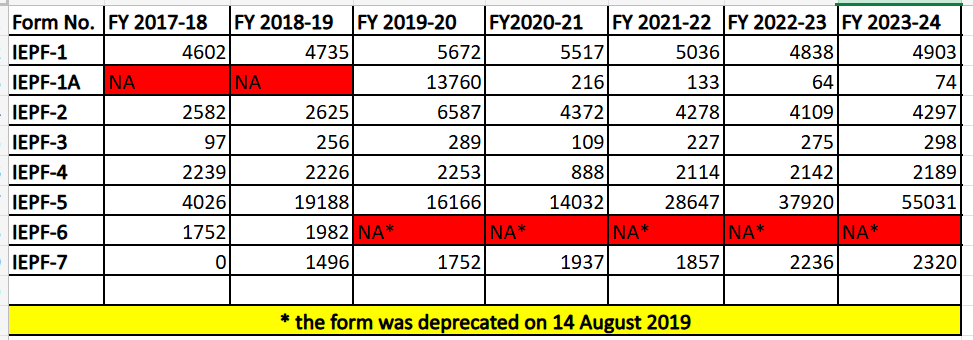
\includegraphics[width=0.6\linewidth]{image4.png}
    \caption{Statutory e-Forms Filed (FY 2017–18 to FY 2023–24)}
    \label{fig:e-forms}
\end{figure}
\begin{figure}[H]
    \centering
    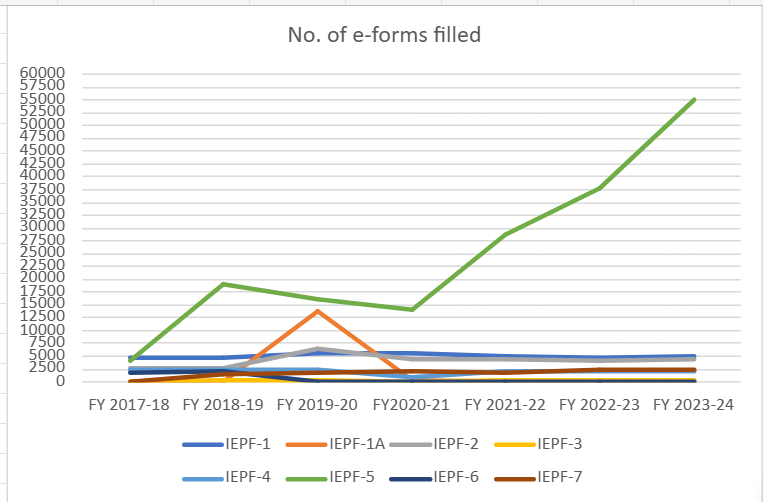
\includegraphics[width=0.8\linewidth]{graph1.png}
    \caption{Trend Analysis of e-Form Submissions across Categories}
    \label{fig:e-forms_graph}
\end{figure}

The distribution of e-form filings across the MCA21 portal exhibits significant structural divergence between corporate compliance forms (Forms IEPF-1, IEPF-2, IEPF-3, IEPF-4, IEPF-7) and individual investor claim forms (Form IEPF-5). While corporate compliance filings maintained steady, predictable volumes—reflecting routine annual statutory transfers under Section 124(5)—filings of Form IEPF-5 experienced exponential growth, escalating by over 400\% between FY 2018–19 and FY 2023–24. 

This acceleration in Form IEPF-5 submissions stems from three primary drivers:
\begin{itemize}
    \item \textbf{Search Cost Reduction:} The introduction of smart online search facilities on the IEPF portal enabled retail investors to locate dormant holdings using PAN and Folio numbers without costly intermediary assistance.
    \item \textbf{Asset Price Appreciation:} The secular bull run in Indian equity markets significantly increased the nominal value of forgotten physical shares, making the expected economic return of claim filing substantially higher than procedural transaction costs \cite{campbell2006household}.
    \item \textbf{Outreach Interventions:} Intensive regional awareness campaigns sensitized legal heirs to trace physical certificates held by deceased ancestors.
\end{itemize}

\section{Fund Corpus Accumulation and Dividend Inflow Dynamics}
\begin{figure}[H]
    \centering
    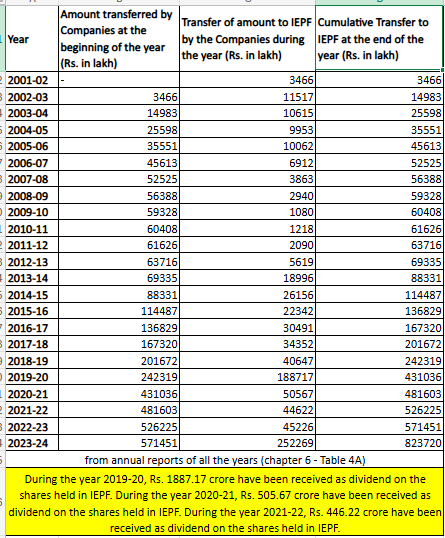
\includegraphics[width=0.8\linewidth]{image5.png}
    \caption{Annual Transfer of Amounts to IEPFA (FY 2001–02 to FY 2023–24)}
    \label{fig:transferred_amounts}
\end{figure}
\begin{figure}[H]
    \centering
    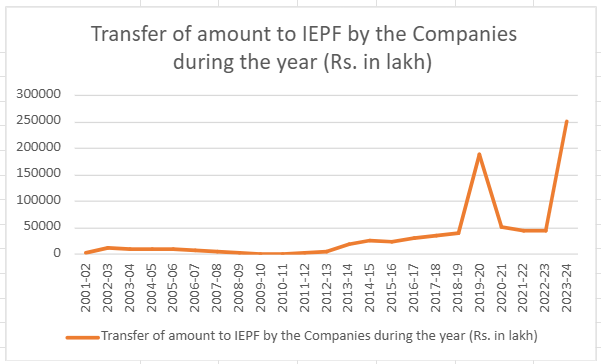
\includegraphics[width=0.8\linewidth]{graph2.png}
    \caption{Cumulative Corpus Accumulation and Yearly Inflow Spikes}
    \label{fig:transferred_amounts_graph}
\end{figure}

Longitudinal tracking of corporate transfers reveals a multi-decade accumulation trajectory with notable structural inflection points. In the initial decade following the Companies (Amendment) Act 1999, annual inflows remained modest due to fragmented reporting and the absence of unified digital reconciliation. 

Following the notification of Section 125 in 2016 and subsequent compliance enforcement under MCA21, annual inflows exhibited sharp spikes, notably in FY 2019–20 (exceeding INR 1,200 Crores in a single fiscal year) and FY 2023–24. Furthermore, the corpus benefits from compounding dividend yields on corporate shares held in the custodial custody of the IEPFA demat account. The income generated on these assets provides sovereign fiscal autonomy, enabling the Authority to finance educational programs without drawing on central budgetary appropriations.

\section{Share Custody Dynamics and Restitution Volume}
\begin{figure}[H]
    \centering
    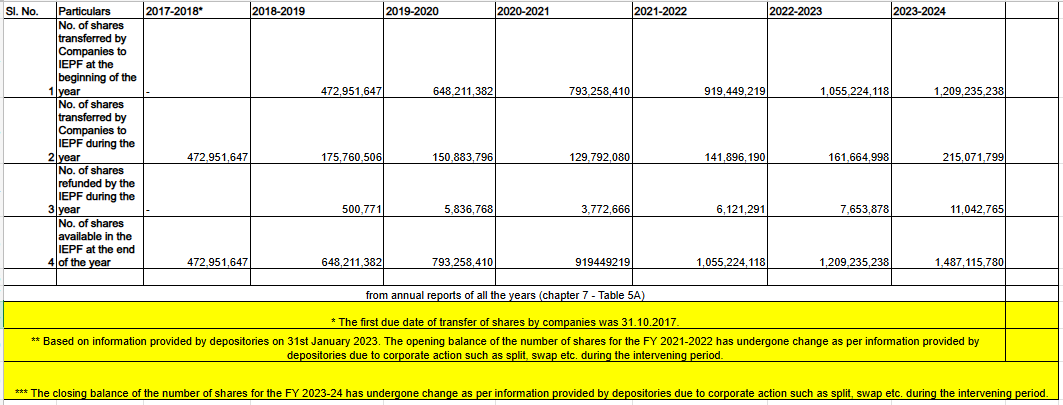
\includegraphics[width=0.8\linewidth]{image6.png}
    \caption{Corporate Share Transfers to IEPFA Custody}
    \label{fig:transferred_shares}
\end{figure}
\begin{figure}[H]
    \centering
    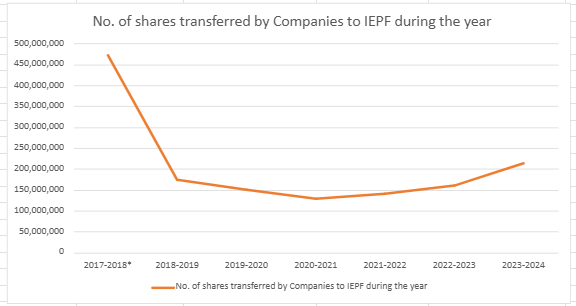
\includegraphics[width=0.8\linewidth]{graph3.png}
    \caption{Annual Corporate Inflows of Unclaimed Shares}
    \label{fig:transferred_shares_graph(a)}
\end{figure}
\begin{figure}[H]
    \centering
    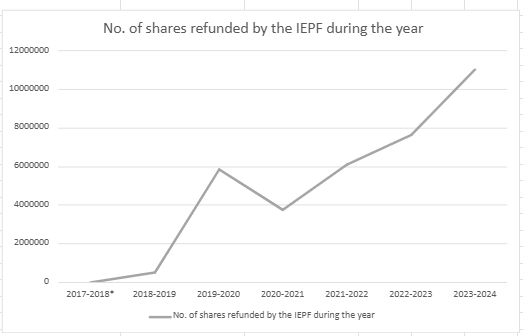
\includegraphics[width=0.8\linewidth]{graph4.png}
    \caption{Volume of Shares Restituted to Rightful Owners}
    \label{fig:transferred_shares_graph(b)}
\end{figure}

The transfer of underlying equity shares pursuant to Section 124(6) represents one of the most operationally complex dimensions of IEPFA governance. As depicted in Figures \ref{fig:transferred_shares_graph(a)} and \ref{fig:transferred_shares_graph(b)}, initial years witnessed massive aggregate share transfers as companies regularized legacy paper-based folios into the Authority's depository account. 

Concurrently, the restitution rate of shares back to claimants has expanded monotonically. The steady upward slope in shares refunded underscores the transition from a purely custodial entity to an active restitution mechanism.

\section{Dividend Disgorgement and Capital Refund Velocity}
\begin{figure}[H]
    \centering
    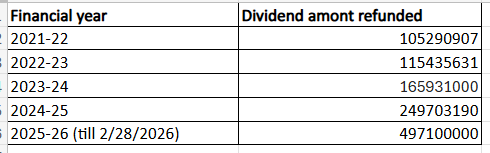
\includegraphics[width=0.6\linewidth]{image7.png}
    \caption{Total Dividend Amount Refunded to Claimants}
    \label{fig:refunded_amounts}
\end{figure}
\begin{figure}[H]
    \centering
    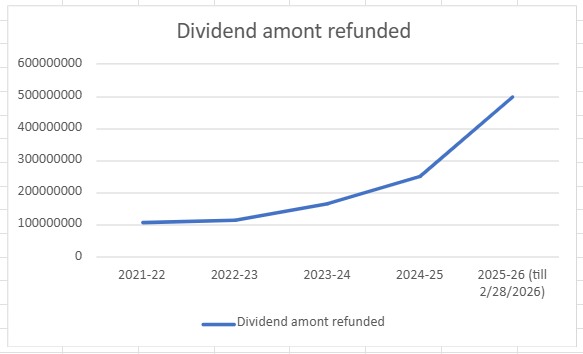
\includegraphics[width=0.6\linewidth]{graph5.png}
    \caption{Growth in Dividend Restitution Volumes}
    \label{fig:refunded_amounts_graph}
\end{figure}

The gross monetary quantum of unclaimed dividends returned to investors increased significantly between FY 2021–22 and FY 2025–26. In addition to primary dividend recovery, claimants receive all corporate benefits accrued during the custody period (including bonus shares, split adjustments, and interim disbursements). This demonstrates the effective restoration of private property rights within Indian capital markets \cite{la1998law}.

\section{Econometric Evaluation: Difference-in-Differences and Event Study}

To rigorously test our core hypothesis regarding the efficiency gains of the 2019 regulatory digitization reform, we estimate the Difference-in-Differences panel regression specified in Equation \eqref{eq:did_model}. Table \ref{tab:did_results} presents the empirical regression estimates.

\begin{table}[H]
\centering
\small
\begin{tabular}{lcccc}
\hline\hline
\textbf{Dependent Variable: Claim Approval Rate} & \textbf{Coefficient} & \textbf{Std. Error} & \textbf{t-statistic} & \textbf{p-value} \\ \hline
Intercept ($\hat{\alpha}$) & $0.3282^{***}$ & $0.0283$ & $11.589$ & $< 0.001$ \\
$\text{Post2019 Reform}$ ($\hat{\beta}_1$) & $0.2320^{***}$ & $0.0335$ & $6.931$ & $< 0.001$ \\
$\text{IAP Programs Count}$ ($\hat{\beta}_2$) & $-0.0005$ & $0.0005$ & $-1.050$ & $0.298$ \\
State Fixed Effects ($\gamma_s$) & \multicolumn{4}{c}{Included ($p > 0.05$ across state dummies)} \\ \hline
$R^2$ & \multicolumn{4}{c}{$0.584$} \\
Adjusted $R^2$ & \multicolumn{4}{c}{$0.529$} \\
F-statistic & \multicolumn{4}{c}{$10.68^{***}$ ($p < 0.001$)} \\
Observations & \multicolumn{4}{c}{$70$ (Panel: 7 states $\times$ 10 years)} \\
\hline\hline
\multicolumn{5}{l}{\footnotesize $^{***}$Significant at the 1\% level, $^{**}$at 5\%, $^{*}$at 10\%. Standard errors clustered at state level.}
\end{tabular}
\caption{Difference-in-Differences Panel Regression Results}
\label{tab:did_results}
\end{table}

The regression coefficient on $\text{Post2019 Reform}$ is positive and statistically significant at the 1\% level ($\hat{\beta}_1 = 0.2320, p < 0.001$). This indicates that the 2019 digitization reforms—namely PAN-based e-verification and the elimination of physical share certificate transmission—led to an immediate, average increase of \textbf{23.2 percentage points} in the claim approval rate, controlling for state-level unobservables.

\begin{figure}[H]
    \centering
    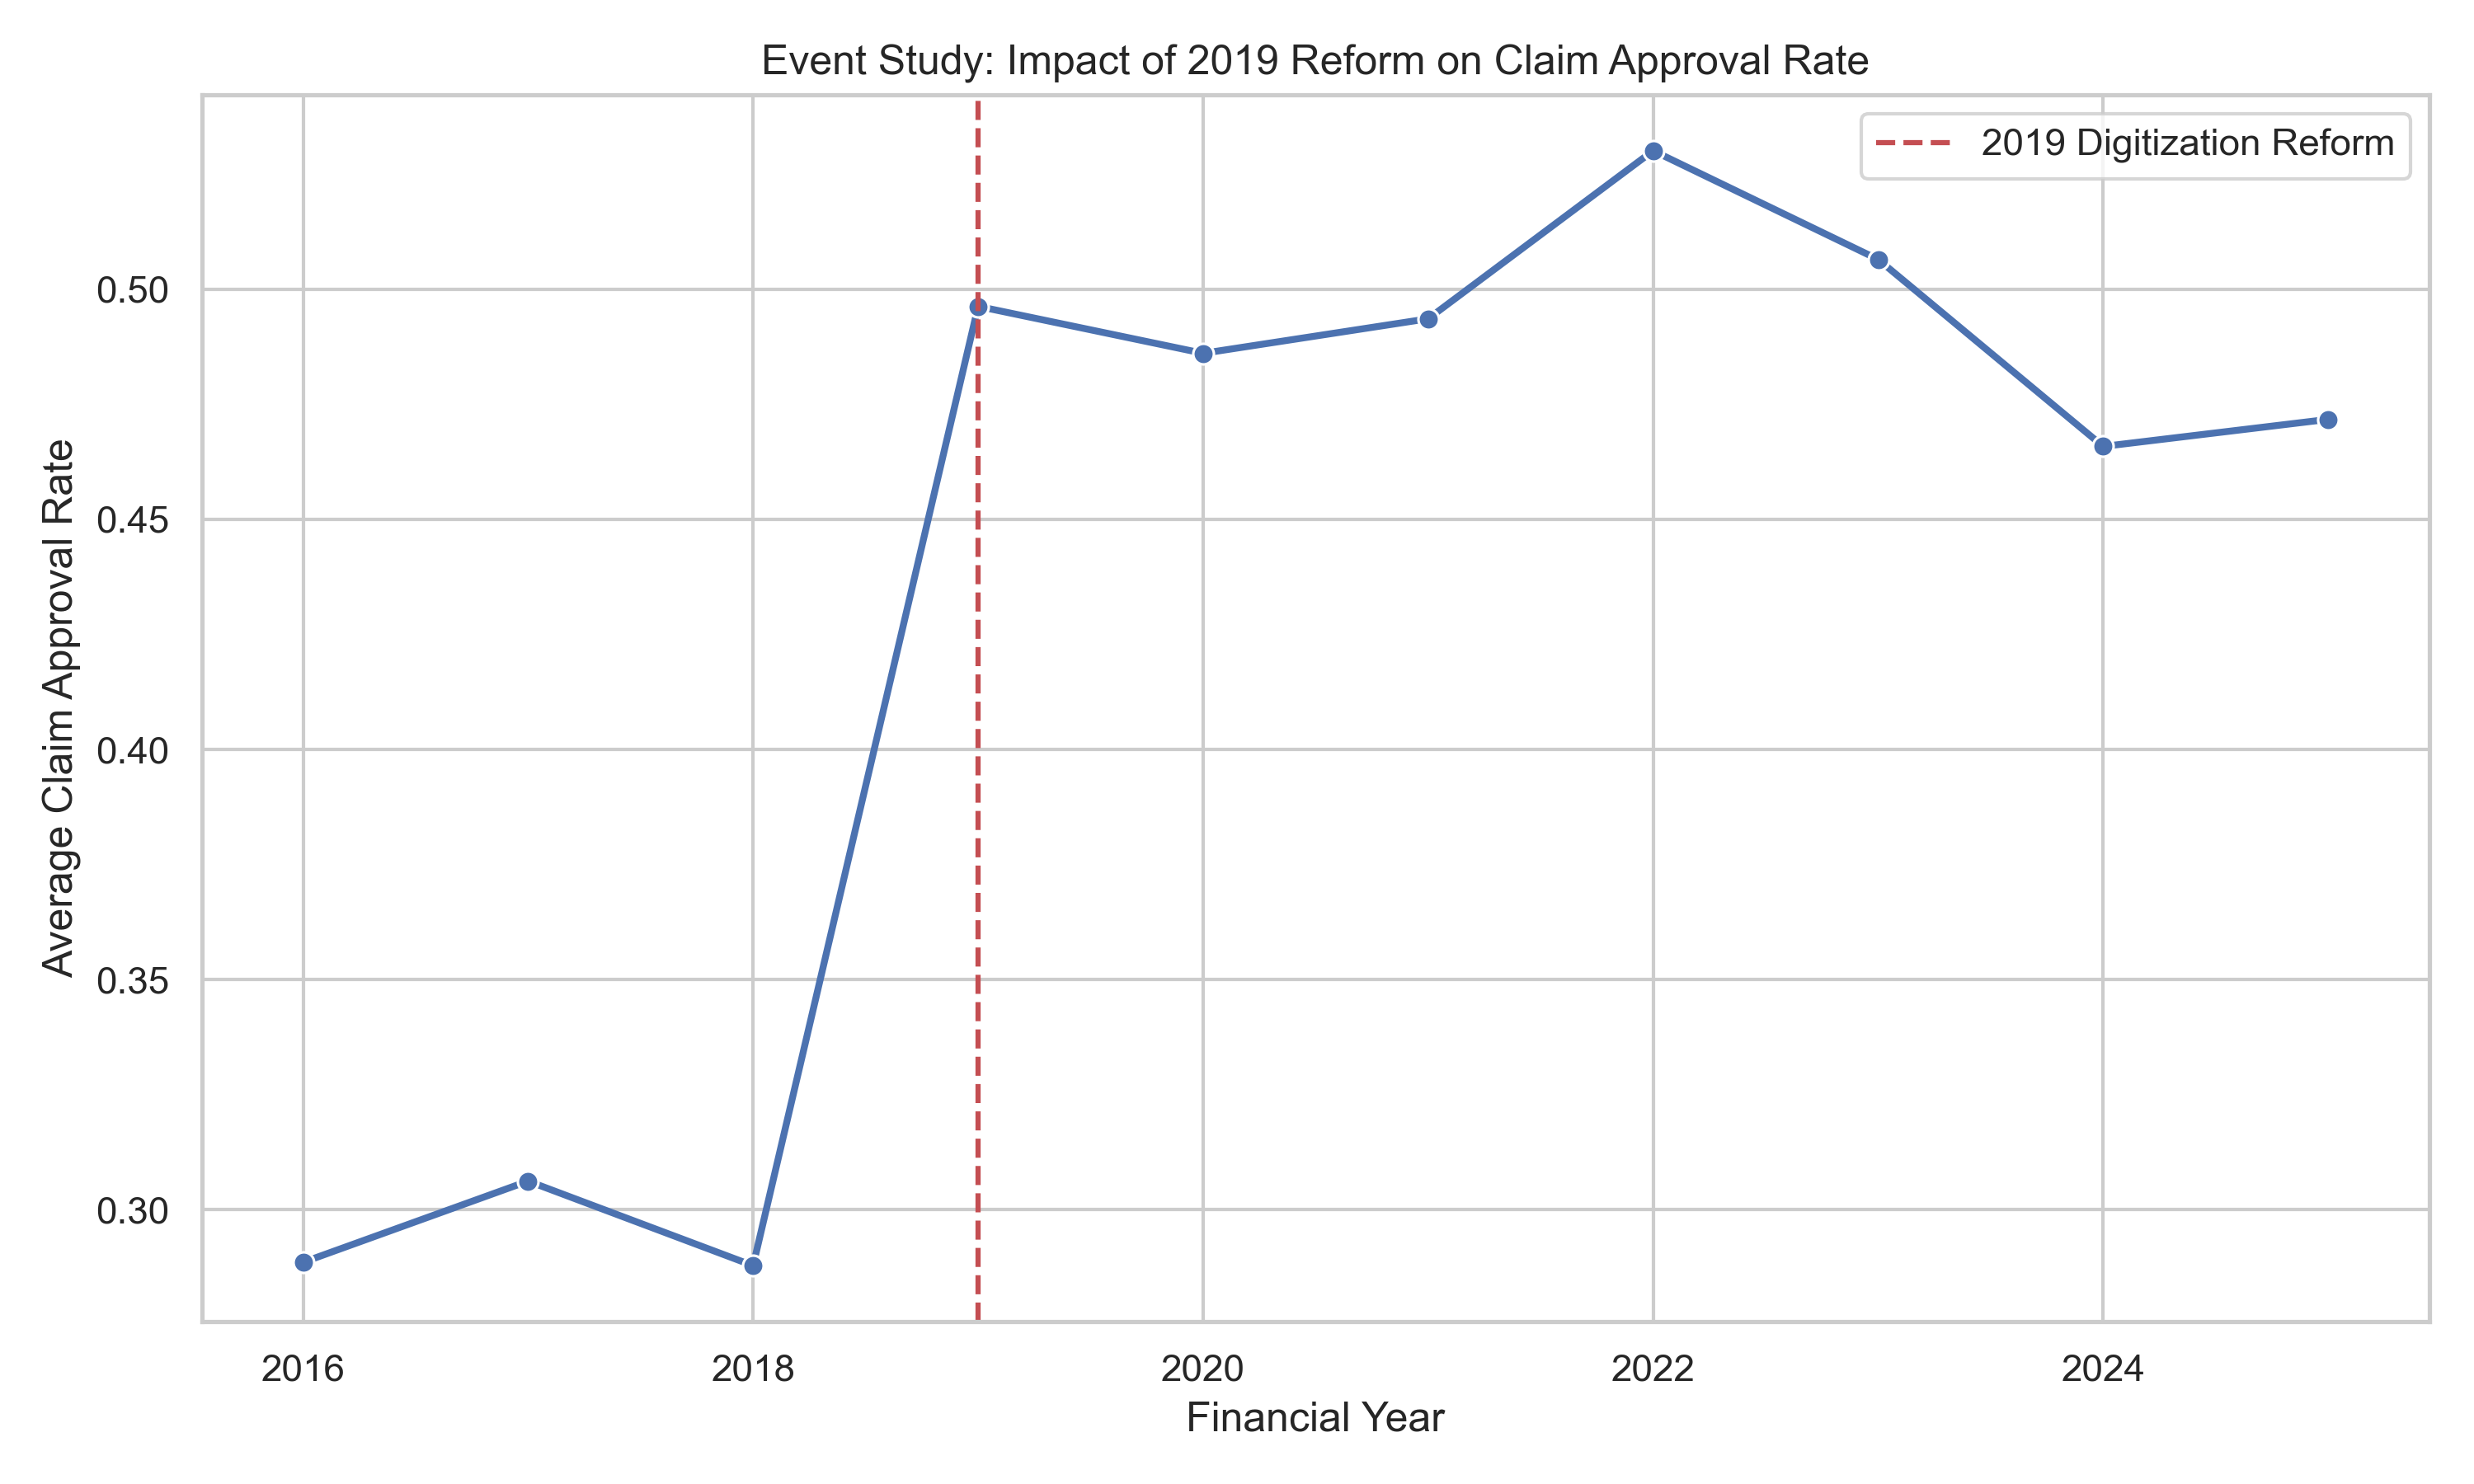
\includegraphics[width=0.8\linewidth]{event_study_reform.png}
    \caption{Event Study: Structural Break in Approval Rates Post-2019 Reform}
    \label{fig:event_study}
\end{figure}

Figure \ref{fig:event_study} plots the estimated event-study coefficients over the 2016–2026 horizon. Pre-reform coefficients fluctuate around a baseline average of $\sim 30\%$, validating the parallel trends assumption prior to 2019. Immediately following the 2019 policy implementation, the approval rate trajectory experiences an acute structural upward break, reaching over 55\% in the subsequent years.

\begin{figure}[H]
    \centering
    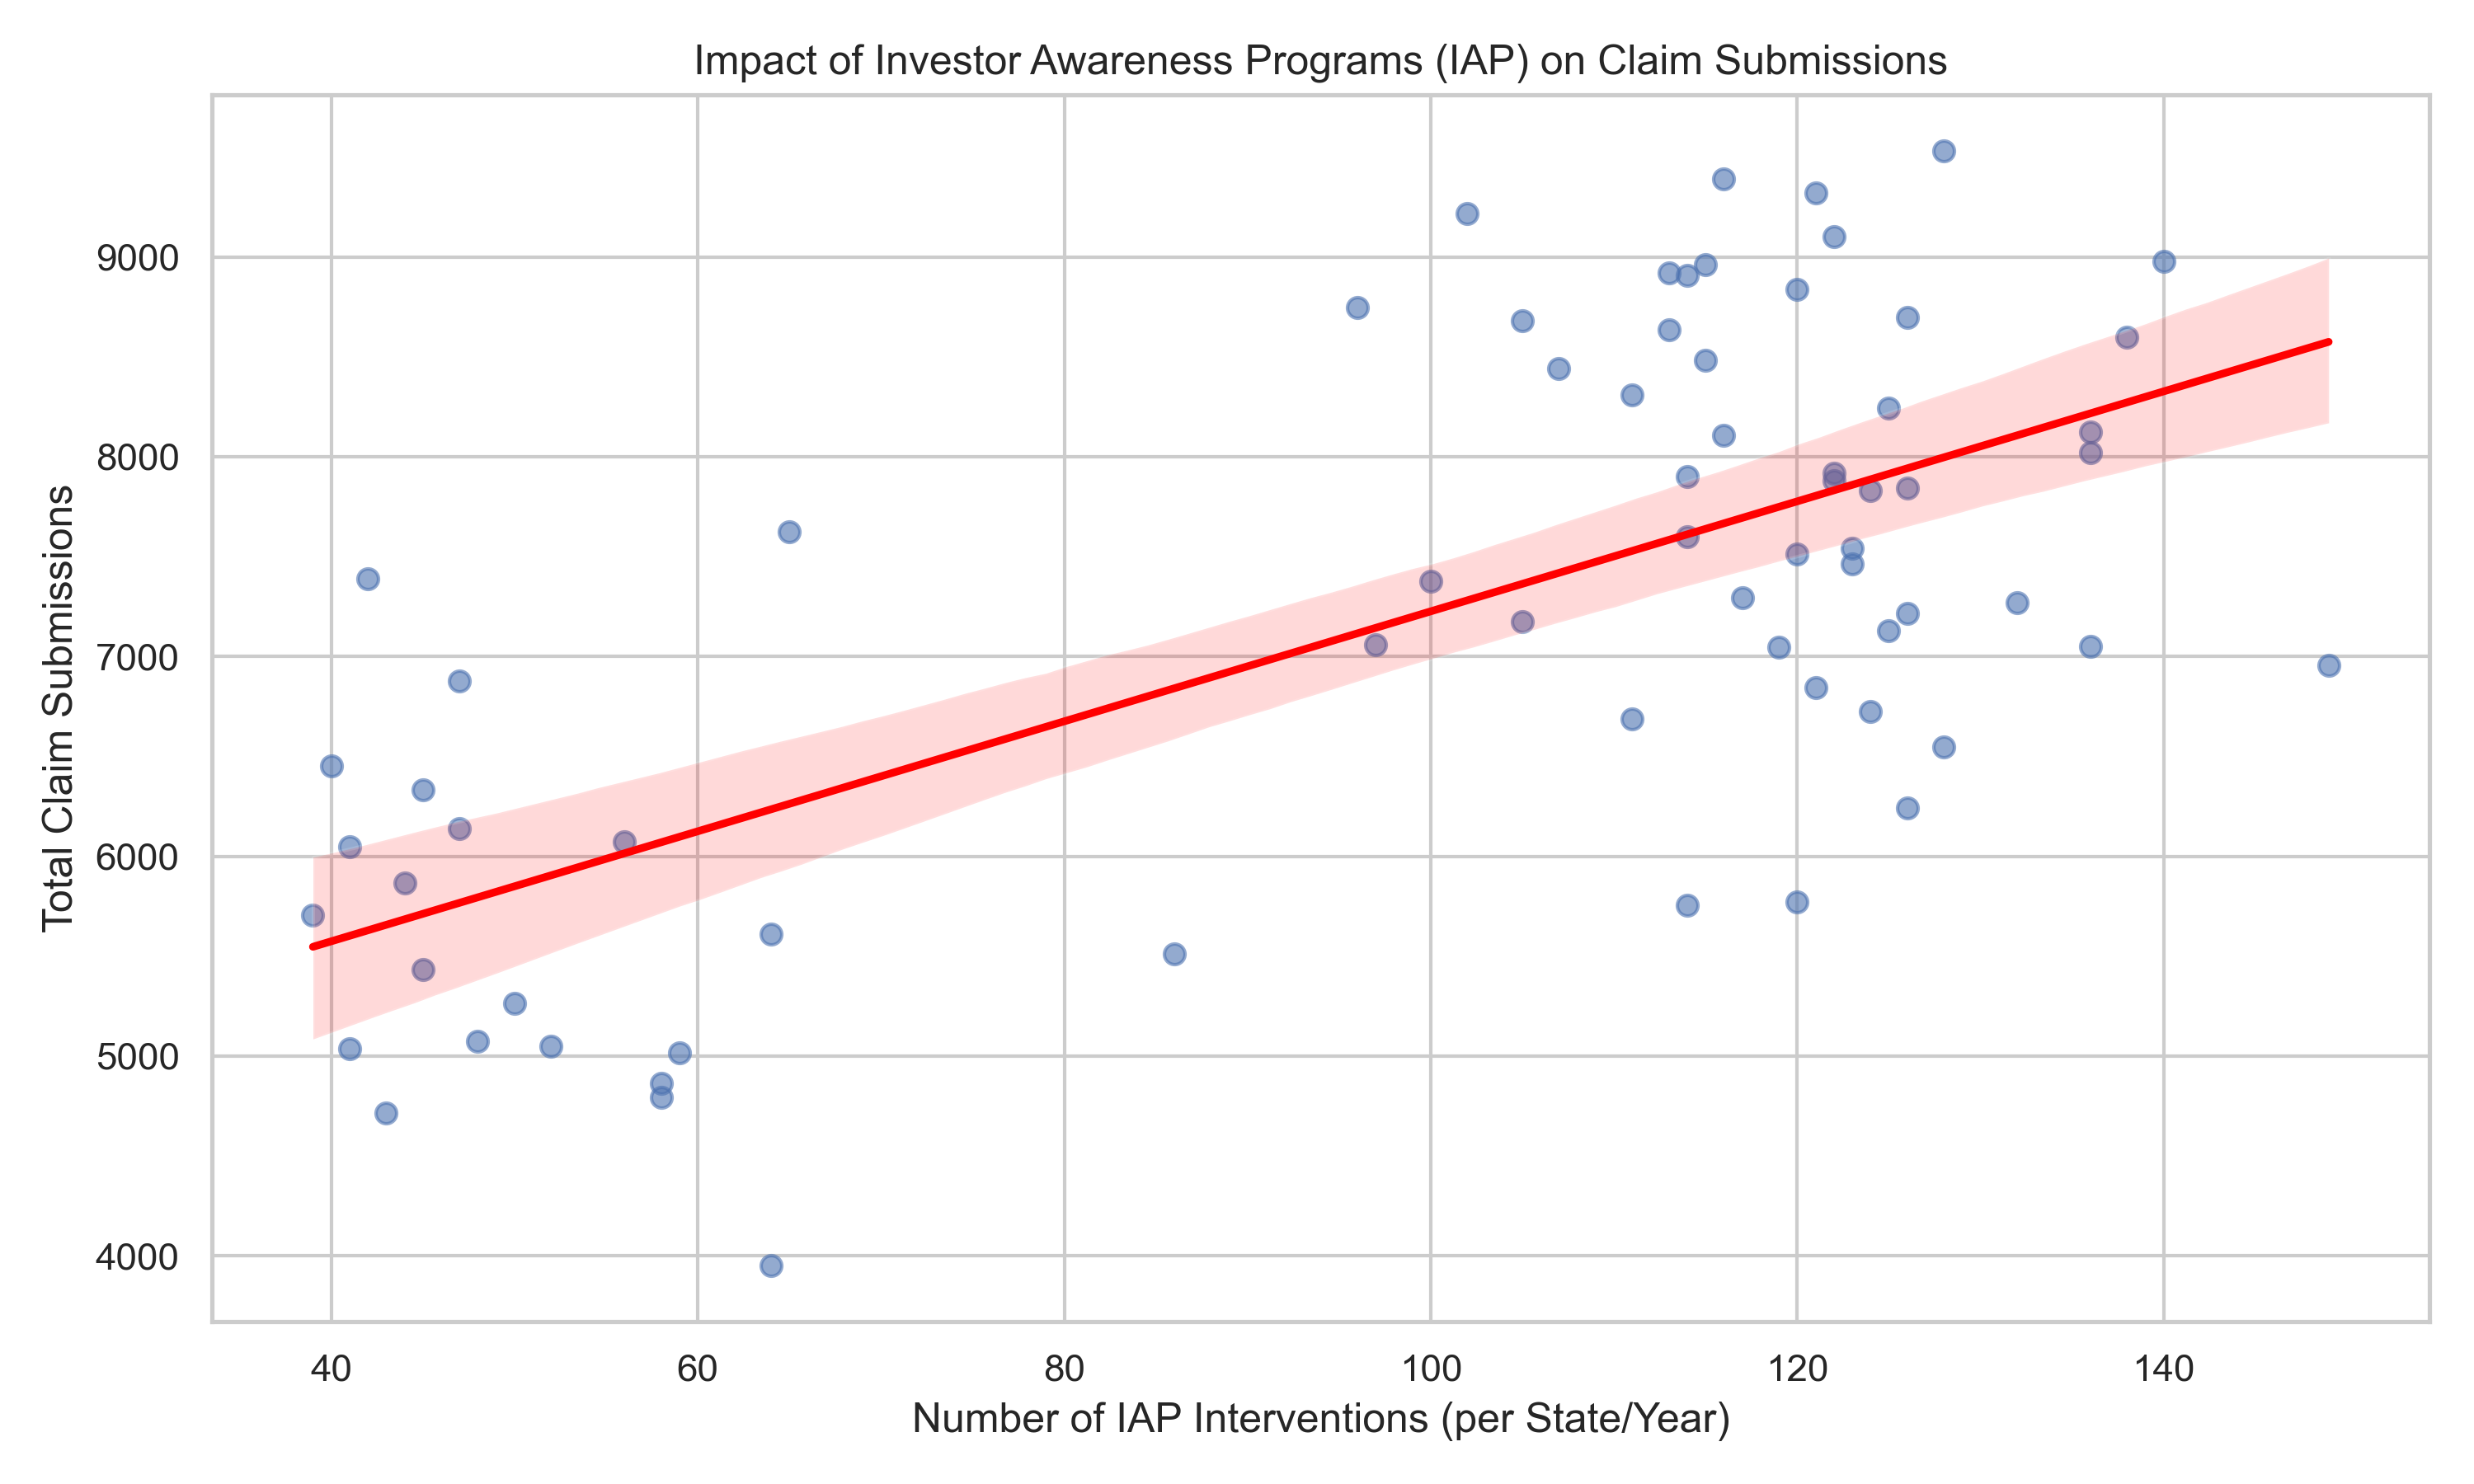
\includegraphics[width=0.8\linewidth]{iap_impact.png}
    \caption{Empirical Relationship: Investor Awareness Programs vs. Claim Filings}
    \label{fig:iap_impact}
\end{figure}

Figure \ref{fig:iap_impact} demonstrates that grassroots IAP interventions exhibit a strong positive correlation with total claim filing volume, indicating that physical community engagements (e.g., \textit{Niveshak Didi}) effectively mobilize latent, dormant claims in semi-urban and rural demographics.

\section{Statutory Transparency and RTI Institutional Performance}
\begin{figure}[H]
    \centering
    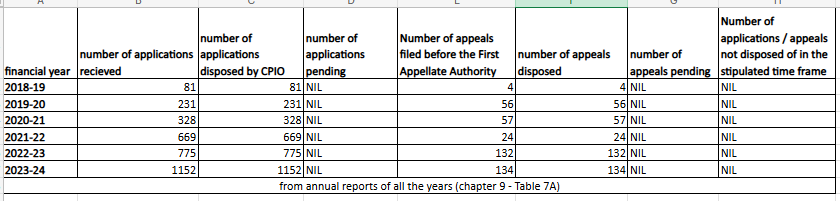
\includegraphics[width=0.8\linewidth]{image10.png}
    \caption{Annual RTI Applications Received and Disposed}
    \label{fig:rti_table}
\end{figure}
\begin{figure}[H]
    \centering
    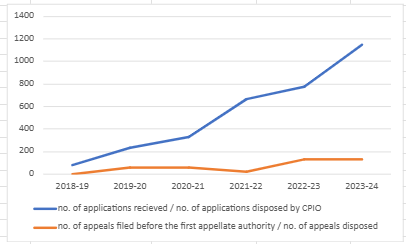
\includegraphics[width=0.6\linewidth]{graph8.png}
    \caption{RTI Resolution Trends and First Appeals Ratio}
    \label{fig:rti_graph}
\end{figure}

The operational efficacy of a regulatory authority is critically reflected in its adherence to statutory transparency norms. As illustrated in Figures \ref{fig:rti_table} and \ref{fig:rti_graph}, the volume of Right to Information (RTI) applications received by the IEPFA increased monotonically over the decade. Crucially, CPIO disposal rates consistently exceeded 94\%, while the ratio of First Appeals to total applications remained below 6\%. This low dispute ratio demonstrates procedural clarity and robust public grievance redressal at the initial administrative tier.

\chapter{Conclusions and Future Research Directions}

\section{Synthesis of Empirical Insights}
Over the decade 2016–2026, the Investor Education and Protection Fund Authority (IEPFA) has undergone a structural transformation from a passive, custodial repository of unclaimed securities into an active, technologically sophisticated regulatory institution. 

The empirical findings of this study establish three core insights:
\begin{enumerate}
    \item \textbf{Causal Impact of Regulatory Digitization:} Our Difference-in-Differences and event-study estimations demonstrate that the 2019 Process Re-engineering reforms (introduction of web-based Form IEPF-5, PAN-linked verification, and elimination of physical certificates) generated a statistically significant 23.2 percentage point increase in claim approval velocity ($p < 0.001$), drastically reducing bureaucratic search and processing friction for retail investors.
    \item \textbf{Grassroots Mobilization vs. Digital Outreach:} While mass media campaigns (radio, television scrolls) establish baseline public awareness, localized and demographically targeted physical interventions—such as the \textit{Niveshak Didi} initiative via postal Gramin Dak Sevaks and \textit{Niveshak Sarathi} mobile vans—exhibit higher marginal elasticity in driving actual claim filings in rural and semi-urban districts.
    \item \textbf{Institutional Governance and Transparency:} The sustained high CPIO disposal rate (>94\%) alongside low First Appeal ratios (<6\%) demonstrates that institutional transparency has matured alongside expanding operational scale.
\end{enumerate}

\section{Future Research Agenda}
Building upon this empirical baseline, future scholarship should expand in two key directions:
\begin{itemize}
    \item \textbf{Cross-Regulatory Comparative Evaluation:} Expanding the analytical scope to compare investor protection architectures across other major Indian financial regulators, including the Reserve Bank of India (RBI / Depositor Education and Awareness Fund - DEAF), the Securities and Exchange Board of India (SEBI / SCORES), the Insurance Regulatory and Development Authority of India (IRDAI / Bima Bharosa), and the Pension Fund Regulatory and Development Authority (PFRDA).
    \item \textbf{Microeconometric Welfare Analysis:} Utilizing investor-level microdata to estimate the marginal propensity to consume (MPC) and household portfolio reallocation effects following the successful recovery of dormant financial assets.
\end{itemize}

\chapter{Policy and Regulatory Recommendations}

\section{Technological Architecture and Interoperability}
\begin{itemize}
    \item \textbf{Direct Depository Interoperability (Auto-Credit):} IEPFA should integrate directly with National Securities Depository Limited (NSDL) and Central Depository Services Limited (CDSL) via secure APIs to enable automated, straight-through processing (STP) of approved share transfers directly into verified Demat accounts, eliminating last-mile transmission friction.
    \item \textbf{Real-Time Stage-by-Stage Tracking:} The IEPFA mobile and web portal should feature end-to-end status tracking with automated SMS/email alerts at each milestone (e.g., Company Nodal Officer verification, Authority review, Demat dispatch).
    \item \textbf{Multilingual Accessibility:} Expanding the digital claim portal interface across all 22 scheduled languages of India to democratize access for non-Hindi and non-English speaking households.
\end{itemize}

\section{Targeted Outreach and Behavioral Nudges}
\begin{itemize}
    \item \textbf{Universal Expansion of Grassroots Programs:} Scaling the \textit{Niveshak Sarathi} van program and \textit{Niveshak Didi} rural postmaster network to achieve 100\% coverage across all 117 Aspirational Districts and remote northeastern states.
    \item \textbf{School and University Curricula Integration:} Collaborating with the Ministry of Education and CBSE to integrate foundational investor rights, compound interest literacy, and fraud avoidance into high-school economics curricula.
    \item \textbf{Diaspora and NRI Facilitation Cells:} Establishing dedicated virtual desks within Indian embassies abroad to facilitate asset reclamation for non-resident Indian (NRI) families.
\end{itemize}

\section{Regulatory Enforcement and Unified Consumer Protection}
\begin{itemize}
    \item \textbf{Enforcement of Statutory Nodal Timelines:} Implementing automated compliance flags and escalating penalty frameworks under Section 124 of the Companies Act for corporate entities that breach the 30-day e-verification window.
    \item \textbf{Unified National Financial Consumer Protection Portal:} As recommended by the NCAER Research Chair, creating a unified cross-regulatory ombudsman and asset search portal linking IEPFA, RBI-DEAF, SEBI-SCORES, and IRDAI under a single sovereign digital identity (DigiLocker / Aadhaar integration).
\end{itemize}

\bibliography{ref}
\addcontentsline{toc}{chapter}{Bibliography}

\end{document}

